\chapter{静态有向模型}
\label{chap:pgm-static-directed}

前三部分分别讲清了概率图模型的三件事：怎样用图\emph{表示}联合分布、给定图后怎样做\emph{推断}、以及怎样从数据\emph{学习}参数和结构。从本章开始的第四部分“模型”，要把这些工具组装到一个个具体的、有名有姓的模型上：每一种模型选定一种图结构和一族局部条件分布，前面学到的推断与学习算法就落到这张具体的图上。本章先从最基础也最常用的一类——\emph{静态有向模型}入手。“静态”指记录之间没有真实的时间先后假设，每条记录是某个时刻拍下的一张“快照”；“有向”指联合分布被写成一串局部条件概率的乘积。

同一个“多个传感器读数常常一起变化”的现象，其实可以在三个层次上追问，而这三个层次恰好对应本章的三条主线。最直接的一层是\emph{观测之间的依赖}：给定第一个读数，第二个读数如何分布（朴素贝叶斯、自回归模型）。更深一层是\emph{记录内部的潜在解释}：两个读数一起升高，会不会是因为背后有一个我们没直接测到的“工作状态”在共同驱动它们（混合模型、因子模型）。再往上，当记录来自不同工厂、不同文档时，还要问\emph{跨记录的共享}：哪些规律是各组通用的、哪些允许各组各自不同（层次模型、主题模型）。

两个传感器的读数经常一起升高。可以直接建模第二个读数在第一个读数给定时的分布，也可以引入未观测的工作状态，让它共同影响两个读数。前一种方法拟合观测间的条件关系，后一种方法还要推断工作状态，并将它从联合分布中汇总掉。若记录又来自不同工厂，还要说明哪些规律跨厂共享、哪些参数允许各厂不同。本章围绕观测间的直接依赖、记录内部的潜在解释和跨记录的共享，分析它们怎样决定学习目标、缺失值查询及相关性的解释。

有向模型将联合分布写成局部条件概率的乘积，概率语义见第~\ref{chap:pgm-directed}章。本章选取静态模型，展开这些局部函数以及相应的推断和学习计算。这里的依赖没有沿真实时间演化的假设。一条记录记为$\bm x\in\mathbb R^d$或离散取值向量，训练数据为$\bm x_1,\ldots,\bm x_n$，待估参数统一记为$\bm\theta$；有类别标签时，用$Y$表示图中的类别节点。

先从全部建模变量都可观测的直接分解开始，再加入离散或连续的潜变量，分析求和与积分怎样形成观测分布。随后将多个记录按组组织，说明共享上层变量与每项选择成分的不同结构。潜变量的取值类型和记录间的共享方式可以同时变化，因此模型比较分别考察这两类选择，以及它们带来的计算和解释代价。

\section{静态观测的有向建模问题}
\label{sec:pgm-static-directed-common}

本节固定全章反复使用的记号和两条共同计算：有向图怎样给出联合分布，以及引入潜变量后似然和后验为何都变成对潜变量的求和或积分。后续具体模型都是在这两条公式上选定不同的图结构和局部函数。记全部节点变量为$\bm V=(V_1,\ldots,V_m)$，图为$\mathcal G$，$\operatorname{pa}_{\mathcal G}(i)$表示节点$i$的父集，$\bm\theta$汇集局部参数。每个节点的条件分布在父变量固定时归一化，联合分布便按图写成
\begin{equation}
  p_{\bm\theta}(\bm v)
    =\prod_{i=1}^m
       p_{\bm\theta_i}(v_i\mid
          \bm v_{\operatorname{pa}_{\mathcal G}(i)}).
  \label{eq:pgm-static-directed-common-joint}
\end{equation}
离散节点使用条件概率，连续节点使用相应基准测度下的条件密度。无环性让各局部条件分布可以按拓扑序组合；其归一化依据见第~\ref{chap:pgm-directed}章。图规定允许使用哪些父变量，函数形式及参数则决定具体的候选分布，二者共同影响能够表达的观测关系。

如果整条记录中的建模变量都已观测，评价似然只需将记录代入这些局部条件分布。若将变量分成观测量$\bm X$和潜变量$\bm Z$，记录只提供$\bm x$，就要汇总所有可能的潜在解释：
\begin{equation}
  \begin{aligned}
    p_{\bm\theta}(\bm x)
      &=\int p_{\bm\theta}(\bm x,\bm z)
                    \,\mathrm d\mu_Z(\bm z),\\
    p_{\bm\theta}(\bm z\mid\bm x)
      &=\frac{p_{\bm\theta}(\bm x,\bm z)}
                    {p_{\bm\theta}(\bm x)}.
  \end{aligned}
  \label{eq:pgm-static-directed-common-marginal}
\end{equation}
$\mu_Z$在离散状态上取计数测度，因此积分表示求和；混合状态则采用对应的乘积测度。后验式要求观测边缘概率或密度为正。第一个式子用于评价观测似然，第二个式子用于判断一条记录的潜在状态；有向分解容易求值，并不意味着这两个汇总都容易计算。

设$n$条记录相互独立并使用同一组固定参数，观测对数似然是各记录对数概率或密度的和：
\[
  \ell(\bm\theta)=\sum_{j=1}^n\log p_{\bm\theta}(\bm x_j).
\]
参数学习需要提高这些记录的概率或密度；含潜变量时，后验期望可能参与EM或梯度计算，通用方法见第~\ref{chap:pgm-parameter-learning}章。一个共享随机上层变量还会在被积分掉后诱导记录间依赖，此时应评价整组记录的联合似然，不能继续套用独立记录的对数似然和。

下面的直接模型限制观测之间的父集或局部函数；有限混合与连续因子模型加入记录内部的潜在解释；层次与混合成员模型进一步规定组间共享和组内分配。它们改变的是不同层次的关系，可以组合使用。这里的箭头表达概率分解，不自动赋予因果含义；变量顺序也不等同于真实时间的演化。

\section{观测之间的直接依赖建模}
\label{sec:pgm-static-directed-direct}

给定一条完整记录，就能在各节点读取父变量的取值，并计算局部条件概率的乘积。局部分布各自归一化后，这个乘积已经是合法的联合分布。缺失某些取值时，还需对它们求和或积分，计算规模随缺失模式改变。这里不为解释记录额外加入随机状态，而是直接规定训练中可见节点的条件分布。类别已记录时，重点是类别内部的属性关系；没有指定类别时，重点是沿所选字段顺序描述完整记录密度。预测时类别未知，只改变查询，不会把训练中已观测的类别改称模型主动引入的潜变量。

\subsection{基于类别条件的属性建模}
\label{sec:pgm-static-directed-naive-tan}

类别条件建模需要在每个类别内估计读数规律。若直接存储全部属性组合，每类的条件表随属性数量迅速增长；先限制类内依赖，再在必要时保留一部分依赖，可以明确控制需要从数据估计的内容。

\subsubsection{朴素贝叶斯：用类内独立减少待估参数}
\label{sec:pgm-static-directed-naive}

给定设备类别和一批传感器读数，最自然的分类问题是：看到读数后，它属于哪一类的可能性最大？要直接估计“读数组合$\to$类别”的完整分布，需要列出所有属性组合的概率，属性一多，组合数指数爆炸、数据根本不够分。一个大胆而朴素的简化是：一旦把类别固定下来，就假设各个读数之间\emph{条件独立}——也就是认为同一类设备的各传感器读数是在类别已知后彼此独立地产生的。这个假设在现实中很少严格成立，却能把一个高维联合分布拆成若干一维分布的乘积，参数量和数据需求骤降，而且实践中分类效果常常出奇地好，这就是朴素贝叶斯。训练数据同时记录设备类别与传感器读数时，可以先估计各类的读数分布，再据新读数计算类别后验。\term{朴素贝叶斯}（naive Bayes, NB）让类别成为所有属性的父节点，给定类别后，各属性共同独立。记$Y$有$K$类，先验为$\pi_k=p(Y=k)$，则
\begin{equation}
  \label{eq:pgm-static-directed-naive}
  p(y,\bm{x})=\pi_y\prod_{i=1}^{d}p(x_i\mid y),\qquad
  p(y\mid\bm{x})=
  \frac{\pi_y\prod_i p(x_i\mid y)}
       {\sum_{k=1}^{K}\pi_k\prod_i p(x_i\mid k)}.
\end{equation}
给定$Y$时的联合独立性，使各属性条件概率能够一起相乘；消去$Y$以后，共同类别仍可使属性相关。训练记录中的类别已知，最大似然估计分别计算类别比例和类内属性分布。预测新记录时，枚举$K$种类别，再将其权重归一化。此时$Y$是查询目标；模型主动引入的潜在状态与漏记的数据字段，则分别需要后面讨论的潜变量推断和缺失数据处理。

这种结构的学习目标可以直接由带标签记录写出。令训练集为$\mathcal D=\{(y_j,\bm x_j)\}_{j=1}^n$，参数包含类别概率$\bm\pi$和各类的属性参数$\bm\theta_i$，最大化监督联合对数似然
\begin{equation}
  \ell_{\mathrm{NB}}(\bm\pi,\bm\theta)
  =\sum_{j=1}^n\left[\log\pi_{y_j}
       +\sum_{i=1}^d\log p_{\bm\theta_i}(x_{j,i}\mid y_j)\right],
  \qquad \bm\pi\in\Delta^{K-1}.
  \label{eq:pgm-static-directed-naive-objective}
\end{equation}
这里$\Delta^{K-1}$表示$K$个非负分量之和为$1$的概率单纯形，离散条件表的每一行也满足这样的归一化约束。对数把条件乘积分成加和，各表行只读取相应类别和父配置的记录，因此可以分别优化。以下计数更新就是这个目标在二值条件模型下的解，并非另设的分类损失。

二值属性使用$a_{i,k}=p(X_i=1\mid Y=k)$。若类别$k$有$n_k>0$条记录，其中第$i$个属性为$1$的记录有$n_{i,k}^{+}$条，计数给出$\widehat\pi_k=n_k/n$、$\widehat a_{i,k}=n_{i,k}^{+}/n_k$。零计数会使某个条件概率为零，读取该表项的完整记录也随之得到零概率；若为类别概率或某行条件表设Dirichlet先验$\operatorname{Dirichlet}(\bm a)$、$a_s>0$，后验预测概率为$(n_s+a_s)/(N+\sum_r a_r)$，其中$N$是该行总计数。这个后验预测规则给未出现的状态保留正质量；它与最大后验估计所用的$a_s-1$修正不同。类别或父配置从未出现时，需要借助先验或其他约束估计其条件表。连续读数可采用类内高斯密度等函数，分布假设随之改变。

对两个类别和二值属性，在所有$a_{i,k}$及先验均严格位于$(0,1)$时，取伯努利似然的对数后验比，得到
\begin{equation}
  \label{eq:pgm-static-directed-naive-boundary}
  \begin{aligned}
  \log\frac{p(Y=1\mid\bm{x})}{p(Y=0\mid\bm{x})}
    &=b+\sum_{i=1}^{d}w_i x_i,\\
  b&=\log\frac{\pi_1}{\pi_0}
       +\sum_i\log\frac{1-a_{i,1}}{1-a_{i,0}},\\
  w_i&=\log\frac{a_{i,1}(1-a_{i,0})}
                       {a_{i,0}(1-a_{i,1})}.
  \end{aligned}
\end{equation}
这条线性评分来自伯努利条件概率的对数比。高斯属性若类间方差不同，对数比会带平方项；一般离散属性则以各状态的指示特征形成加性评分。NB先估计生成分布再得到系数，直接拟合分类损失则从类别预测目标估计系数，两者的学习方式不同。

\begin{example}[两个二值读数]
  \label{ex:pgm-static-directed-binary}
  另取一组人工参数，比较两个读数的直接分解与潜在解释。用$Y=1$表示异常工作状态，$X_1,X_2$表示二值读数，设
  \[
  \begin{gathered}
    p(Y=1)=0.1,\\
    p(X_1=1\mid Y=1)=0.8,\quad
    p(X_1=1\mid Y=0)=0.1,\\
    p(X_2=1\mid Y=1)=0.7,\quad
    p(X_2=1\mid Y=0)=0.2.
  \end{gathered}
  \]
  给定$Y$，两个读数独立生成。对观测$(X_1,X_2)=(1,1)$，两类权重为$0.1\times0.8\times0.7=0.056$与$0.9\times0.1\times0.2=0.018$，归一化得到
  \[
    p(Y=1\mid1,1)=\frac{0.056}{0.074}
      =\frac{28}{37}\approx0.7568.
  \]
  消去类别后，两个读数的边缘概率为$p(X_1=1)=0.17$、$p(X_2=1)=0.25$，联合概率$p(1,1)=0.074$却高于两边缘乘积$0.0425$。协方差为$0.0315$，显示共同类别引起的观测相关。
\end{example}

类内依赖也可能让两个读数重复提供同一信息。令第二个读数完全复制第一个，即$X_2=X_1$，并保持上述先验及$X_1$条件分布；两者为$1$时，正确后验为$0.08/(0.08+0.09)=8/17$。按独立属性重复相乘，却得到$0.064/(0.064+0.009)=64/73$，不仅改变按最大后验作出的类别判断，也放大对该判断的置信度。因此评价这项假设时，需要分别检查分类结果和后验概率。

\subsubsection{树增强朴素贝叶斯：保留一层类内依赖}
\label{sec:pgm-static-directed-tan-model}

复制读数的反例表明，同类内仍有关联的属性不能一概当作独立证据。完全放开父集又会回到庞大的条件表，因此可以先只允许每个属性额外读取一个属性，保留树形的类内依赖。

为了表示类内依赖，可以在类别指向全部属性的结构上，再加入一棵属性树，得到\term{树增强朴素贝叶斯}（tree-augmented naive Bayes, TAN）。选属性$r$为根，将树边从根向外定向，非根属性$i$的属性父节点记为$t(i)$，联合分布为
\begin{equation}
  \label{eq:pgm-static-directed-tan}
  p(y,\bm{x})=
    p(y)p(x_r\mid y)
    \prod_{i\ne r}p(x_i\mid y,x_{t(i)}).
\end{equation}
每个非根属性增加一个属性父节点，给定类别后，各属性按树上的条件概率生成。图~\ref{fig:pgm-static-directed-classifiers}将这棵树与NB结构并列；新增边提供允许建模的依赖，若要解释为因果关系，还需额外的建模依据。

\begin{figure}[htbp]
  \centering
  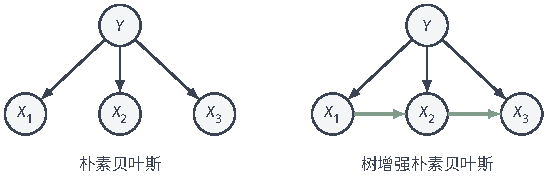
\includegraphics[width=92.650mm]{figures/06-probabilistic-graphical-models/04-models/tikz/pgm-static-directed-classifiers/figure.pdf}
  \caption{类别模型的两种属性结构。NB给定$Y$后各属性独立；TAN增加$X_1\to X_2\to X_3$，使右图的条件分布保留属性树上的依赖。训练时读入类别，预测时根据属性查询类别，观测状态随任务确定。}
  \label{fig:pgm-static-directed-classifiers}
\end{figure}

允许更大的父集，会增加需要估计的条件表。若属性$i$有$r_i$个状态，NB的自由参数为$(K-1)+K\sum_i(r_i-1)$；固定TAN属性树后，按父配置计数得到
\[
  (K-1)+K(r_r-1)
       +K\sum_{i\ne r}r_{t(i)}(r_i-1).
\]
两个类别和三个二值属性的自由参数由NB的$7$个增为TAN的$11$个，仍小于完整联合表所需参数，但新增父配置也需要数据支持。给定完整属性，两个模型枚举类别的评分均需$O(Kd)$次局部查询。二值TAN的对数评分还可含$x_i x_{t(i)}$项，因而能够表示属性间的交互。

TAN的学习包含参数估计与树选择两个层次。记定向后的属性树为$T$，固定它时，最大化
\begin{equation}
  \ell_T=\sum_{j=1}^n\left[
    \log\pi_{y_j}+\log p(x_{j,r}\mid y_j)
    +\sum_{i\ne r}\log p(x_{j,i}\mid y_j,x_{j,t(i)})\right].
  \label{eq:pgm-static-directed-tan-objective}
\end{equation}
每行条件表按类别与属性父值分组计数，再以该行总数归一化。树未知时，还需比较不同$T$各自达到的最大似然；下面把这个比较化成边权之和。选定树后重新按其父配置拟合条件表，便得到可用于类别预测的完整模型。

对于完整离散数据，可以选择使训练似然最大的属性树。先用经验分布$\widehat p$计算给定类别的条件互信息
\[
  \widehat I(X_i;X_j\mid Y)=
  \sum_{y,x_i,x_j}\widehat p(y,x_i,x_j)
  \log\frac{\widehat p(x_i,x_j\mid y)}
                 {\widehat p(x_i\mid y)\widehat p(x_j\mid y)}.
\]
求和只计算正频数项，零频数项以连续延拓取$0$。将候选树上的条件表分别拟合为最大似然表，其平均训练对数似然为
\begin{equation}
  \label{eq:pgm-static-directed-tan-score}
  -\widehat H(Y)-\sum_i\widehat H(X_i\mid Y)
  +\sum_{\{i,j\}\in E_{\mathrm{T}}}
       \widehat I(X_i;X_j\mid Y),
\end{equation}
这里$\widehat H$是经验熵，$E_{\mathrm T}$是属性树的无向边集。每个非根属性的条件熵可写为$H(X_i\mid Y,X_j)=H(X_i\mid Y)-I(X_i;X_j\mid Y)$，根仍贡献$H(X_r\mid Y)$；将各项相加，便得到式中的熵项与树边互信息。熵项不随树改变，因此以条件互信息为边权，求最大生成树并任取根定向即可。这个最大似然结论针对观测完整、无结构惩罚和自由条件表的设定，其他约束需重新分析得分。

若$r_i\le r$，直接统计全部属性对需$O(nd^2)$次计数更新，遍历条件表求边权需$O(Kd^2r^2)$操作，稠密最大生成树需$O(d^2)$时间。NB只统计单属性，计数为$O(nd)$。TAN增加这部分工作以拟合类内依赖，树结构仍限制可表达的高阶相互作用；数据稀疏时，新增条件表和不稳定的树边可能增加估计误差。Friedman等给出了TAN及其算法，结构学习的一般得分推导见第~\ref{chap:pgm-structure-learning}章\scite{pgm-static-directed-friedman1997}

\subsection{基于顺序条件的密度建模}
\label{sec:pgm-static-directed-autoregressive}

朴素贝叶斯需要一个已观测的类别节点来组织条件分布。若手头\emph{没有}类别标签、只想描述一条完整记录本身的联合分布，还有一个对任意联合分布都成立的通用办法：概率链式法则。它让我们人为给变量排一个顺序，然后把“整条记录的概率”写成第一个变量的边缘概率、给定第一个后第二个的条件概率、依此类推各项的连乘。这样做的好处是每一个因子都是一个归一化的条件分布，可以用功能很强的模型（如神经网络）逐个拟合，且无需引入任何潜变量、没有难以计算的积分；代价是要选定一个顺序，而且生成时只能沿该顺序逐个抽样。拟合观测的联合分布时，也可以依次为每个变量建立给定前面变量的条件分布。选定字段或像素的次序，把第$i$位以前的取值记为$\bm x_{<i}$。\term{自回归密度模型}（autoregressive density model）沿这个顺序计算条件概率，再相乘形成
\begin{equation}
  \label{eq:pgm-static-directed-ar}
  p_{\bm{\theta}}(\bm{x})
    =\prod_{i=1}^{d}p_{\bm{\theta}}(x_i\mid\bm{x}_{<i}).
\end{equation}
这种顺序规定预测前缀，例如表格字段排列或图像扫描顺序。第一个前缀$\bm x_{<1}$为空，因此第一项是边缘分布；各字段之间无需具有真实时间关系。

局部归一化保证式~\eqref{eq:pgm-static-directed-ar}的联合分布也归一化。离散变量先对$x_d$求和，最后一项变为$1$；依次消去$x_{d-1},\ldots,x_1$，最后留下$\sum_{x_1}p(x_1)=1$。连续变量使用非负可测、每个前缀下均归一化的条件密度，借助Tonelli定理依次积分，也得到总质量$1$。从某个联合分布恢复条件分布时，零概率前缀可补任意归一化条件分布，它与前缀零权重相乘后仍为零。归一化确定了概率合法性，拟合数据的质量还取决于所选条件函数。

链式法则允许任意联合分布沿任意变量排列分解。对二值变量使用完整条件表，仍需$1+2+\cdots+2^{d-1}=2^d-1$个自由参数。实际用有限宽度网络、有限感受野或高斯条件减少参数时，模型只保留这些局部函数可表达的分布。变量排列会改变待拟合的条件关系：一个方向的条件可能近似单峰，反向却可能出现多个峰，因此同样容量的函数在不同顺序下可产生不同误差。

消去例~\ref{ex:pgm-static-directed-binary}中的类别，得到两个读数的观测联合表
\[
  \begin{array}{ccccc}
    (x_1,x_2)&(0,0)&(0,1)&(1,0)&(1,1)\\
    p(x_1,x_2)&0.654&0.176&0.096&0.074
  \end{array}
\]
以$X_1$在前的顺序，将这张表改写为三个条件参数：
\[
  \begin{aligned}
    p(X_1=1)&=0.17,\\
    p(X_2=1\mid X_1=1)&=\frac{37}{85},\\
    p(X_2=1\mid X_1=0)&=\frac{88}{415}.
  \end{aligned}
\]
例如由$p(X_1=1)=0.17$和$p(X_2=1\mid X_1=1)=37/85$相乘，恢复$p(1,1)=0.074$。直接分解保留了整张读数联合表，用它能预测另一读数。若查询未观测工作状态$Y$，则还需要定义含$Y$的模型；观测表本身只给读数间的关系。

每个输出层需定义当前变量的完整条件分布。二值变量使用伯努利参数，有$r$个状态的变量使用softmax归一化概率；图像通道有$256$个离散值时，可以输出$256$项概率。连续条件可以输出均值$\mu_i(\bm x_{<i})$和正尺度$\sigma_i(\bm x_{<i})$来定义高斯密度，多峰条件则输出有限高斯混合的权重、均值和尺度。局部成分指示可被显式求和，因此混合参数化仍能计算这一条件似然。离散质量与连续密度使用不同的参考测度；将量化像素连续化时，还需给出量化区间积分或去量化方案。

完整训练记录提供每一位真实前缀，对这些条件分布的负对数似然求和，形成
\begin{equation}
  \label{eq:pgm-static-directed-ar-loss}
  L(\bm{\theta})=-\sum_{j=1}^{n}\sum_{i=1}^{d}
      \log p_{\bm{\theta}}
      (x_{j,i}\mid\bm{x}_{j,<i}).
\end{equation}
学习方法是把完整记录代入各条件函数，按式~\eqref{eq:pgm-static-directed-ar-loss}累加梯度，再更新共享参数。用小批量近似全数据梯度时，每个入选记录仍提供各位置的真实前缀。不同网络会采用逐步递推或同时前向计算，但共同优化的是这一个完整记录似然。额外的跨位置计算需要保持相同的读取约束，例如将全部输入汇总后广播到每个输出，会重新引入未来或当前目标信息。

生成记录时，条件所需的前缀尚待抽样。先取$X_1$，再据其结果取$X_2$，沿顺序继续，完成祖先采样。具有完整顺序依赖的标量模型要作$d$轮相继决策，不同记录可以批处理，同一记录则按前缀推进。缓存减少各轮重复计算，但前后状态的依赖仍保留。NB在类别给定后各属性独立，可并行抽样；TAN可按属性树的层次并行，生成顺序因此取决于具体父集。

自回归分解提供可计算的完整似然和顺序采样。观测的是前缀时，余下部分可按原条件分布续写；若第一位缺失、后面的多位已观测，计算第一位的后验可能需要汇总一批变量。选择模型时，应分别评估完整密度、祖先采样和任意条件补全的成本。第~\ref{chap:pgm-generative}章将沿用这条直接似然路线，与其他神经生成构造比较。

\subsubsection{NADE：复用逐步增长的前缀表示}
\label{sec:pgm-static-directed-nade-model}

用完整条件表实现自回归分解时，第$i$个条件分布要读取前面所有变量，参数表大小随$i$指数增长。换成神经网络拟合这些条件函数可以压缩参数量，但如果为每个位置$i$都各训练一个独立网络，又会有$d$个网络、彼此不共享，且无法利用“前$i$个变量的前缀”和“前$i+1$个变量的前缀”高度重叠这一事实。NADE的思路是让所有位置\emph{共用同一个网络}，并利用前缀只比上一步多一个变量的特点做增量计算：算出第$i$个条件所用的隐藏表示后，只需再加一项就能得到第$i+1$个条件的隐藏表示，而不必从头前向。逐前缀条件表的大小随维数增长。\term{神经自回归分布估计器}（neural autoregressive distribution estimator, NADE）让不同前缀共用网络参数，以限制需要保存的参数量。对二值观测，宽度为$h$的单隐藏层条件函数为
\begin{equation}
  \label{eq:pgm-static-directed-nade}
  \begin{aligned}
    \bm{a}_i&=\bm{c}+\sum_{j<i}\bm{W}_{:,j}x_j,&
    \bm{h}_i&=\operatorname{sigmoid}(\bm{a}_i),\\
    p(X_i=1\mid\bm{x}_{<i})
      &=\operatorname{sigmoid}
        (b_i+\bm{V}_{i,:}\bm{h}_i).
  \end{aligned}
\end{equation}
其中$\bm W\in\mathbb R^{h\times d}$、$\bm V\in\mathbb R^{d\times h}$，$\bm c,\bm b$为偏置，$\operatorname{sigmoid}(u)=(1+\exp(-u))^{-1}$。前缀从$i$延长到$i+1$时，用$\bm a_{i+1}=\bm a_i+\bm W_{:,i}x_i$增量更新，成本为$O(h)$；配合每位的输出计算，完整记录评价需$O(dh)$操作。$\bm h_i$由已知前缀确定，可直接计算，无需作为随机潜变量积分。这个前缀复用方式构成NADE计算似然的基础\scite{larochelle2011}

对式~\eqref{eq:pgm-static-directed-nade}输出的概率记$q_{j,i}$，NADE实际最小化的二值目标为
\[
 L_{\mathrm{NADE}}=-\sum_{j,i}
 [x_{j,i}\log q_{j,i}+(1-x_{j,i})\log(1-q_{j,i})].
\]
每轮沿前缀递推得到各$q_{j,i}$，将所有位置的误差信号反向传给共享的$\bm W,\bm V,\bm b,\bm c$，再作梯度更新。生成时把前一步抽得的值接入递推；有限隐藏宽度限制所能表示的条件函数，$O(dh)$计算量本身不保证拟合任意二值联合表。

\subsubsection{MADE：用掩码同时计算合法条件}
\label{sec:pgm-static-directed-made-model}

NADE要沿前缀一步步递推才能算完一条记录的似然，难以借助现代硬件一次性并行。于是产生一个诱人的想法：能不能让网络\emph{一次前向就同时输出}全部$d$个条件分布？难点在于自回归顺序要求“第$i$个输出只能看见前$i-1$个输入”，而普通全连接网络的每个输出能看见所有输入，会作弊地读到自己的当前值。MADE的解决办法非常直接：用一组固定的\emph{掩码}把违反顺序的连接权重强制置零，从结构上保证每个输出读取的恰好是它的合法前缀，从而在一次并行前向中算出全部条件。也可以同时计算各条件，但限制每个输出能读取的输入。\term{掩码自编码分布估计器}（masked autoencoder for distribution estimation, MADE）将违反自回归顺序的连接置零。给输入$j$次序号$j$、隐藏单元$u$次序号$m(u)$，仅保留输入边$j\le m(u)$与输出边$m(u)<i$。深层隐藏边的次序号非递减，输出端仍要求严格小于$i$，故每条输入到输出的路径都满足$j<i$。这样同时算出的第$i$个条件只使用合法前缀。

对单隐藏层二值输出，这些限制落实在权重矩阵上，模型结构可写成
\begin{equation}
  \bm h=\sigma((\bm W\odot\bm M_{\mathrm{in}})\bm x+\bm c),
  \qquad
  \bm q=\sigma((\bm V\odot\bm M_{\mathrm{out}})\bm h+\bm b),
  \label{eq:pgm-static-directed-made-structure}
\end{equation}
其中$\odot$为逐元素相乘，$\sigma$逐元素取sigmoid，$q_i$是第$i$个伯努利条件参数。训练使用与NADE相同的二值负对数似然，一次前向即可评价完整记录各位置；梯度只更新掩码允许的权重。生成时仍需先抽出第$i$位所依赖的前缀，再使用$q_i$，所以并行评价训练似然不等于并行生成整条记录。

图~\ref{fig:pgm-static-directed-mask}取三个输入和两个次序号分别为$1,2$的隐藏单元。以接收端为行、发送端为列，输入与输出掩码为
\[
  \bm{M}_{\mathrm{in}}=
  \begin{pmatrix}1&0&0\\1&1&0\end{pmatrix},\qquad
  \bm{M}_{\mathrm{out}}=
  \begin{pmatrix}0&0\\1&0\\1&1\end{pmatrix}.
\]
矩阵相乘得到$\left(\begin{smallmatrix}0&0&0\\1&0&0\\2&1&0\end{smallmatrix}\right)$，其非零项只在严格下三角，元素$2$计数两条合法路径。第一个条件输出仅用偏置，第三个输入只作为第三位似然的目标值，未进入任何条件参数。普通自编码器允许输出访问当前输入，可以通过复制完成重构。MADE结合前缀掩码与归一化条件输出，用各条件的负对数概率训练联合分布；这种似然目标需要由条件分布定义，普通重构误差则取决于另行选用的输出和损失\scite{pgm-static-directed-germain2015}

\begin{figure}[htbp]
  \centering
  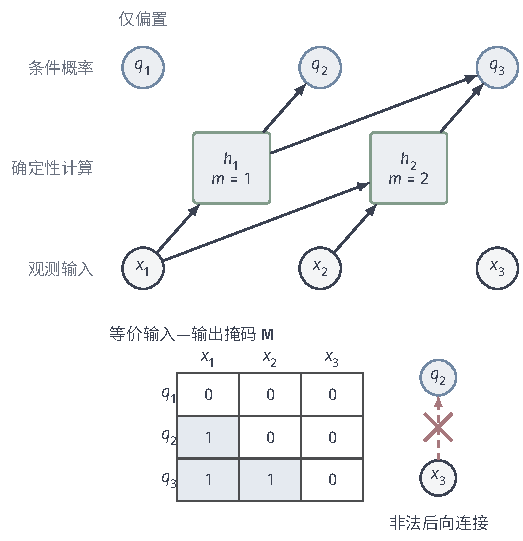
\includegraphics[width=88.554mm]{figures/06-probabilistic-graphical-models/04-models/tikz/pgm-static-directed-mask/figure.pdf}
  \caption{MADE掩码限定的条件依赖。隐藏方框进行确定性计算，输入与输出用圆框表示，$q_i=p(X_i=1\mid\bm x_{<i})$。下方输入—输出掩码中蓝色单元的1标出允许读取的前缀，右侧$x_3\to q_2$展示违反顺序的连接；各隐藏单元的次序号共同保证输出只能读取此前的输入。}
  \label{fig:pgm-static-directed-mask}
\end{figure}

\subsubsection{PixelCNN：把条件网络改为空间共享的掩码卷积}
\label{sec:pgm-static-directed-pixelcnn-model}

NADE、MADE都把输入当作一个没有空间结构的向量。但对图像而言，像素天然排布在二维网格上，同样的边缘、色块等局部图案会在图中不同位置反复出现；若为每个像素位置都单独保存一套连接权重，既浪费参数又无法利用这种“同一图案到处出现”的平移规律。卷积神经网络的优势正是让同一组卷积核在所有空间位置共享。于是只需把MADE的“掩码”思想搬到卷积上：按从上到下、从左到右的扫描顺序，让每个像素的条件网络只能读到它上方的行和同一行左侧的像素，就把空间权值共享与自回归的前缀约束结合起来。图像中相似的局部图案会出现在不同位置。为每个位置分别保存完整连接权重，没有利用这种重复；让相同卷积核在空间上复用，再屏蔽不合法的读取位置，就能把空间共享与前缀约束结合。

对图像，可用卷积共享不同位置的条件函数。\term{像素卷积自回归模型}（PixelCNN）按逐行扫描顺序，用掩码卷积读取当前像素上方和同行左侧的上下文。输入层排除当前目标值，后续层可读取当前位置已由合法前缀形成的隐藏表示。彩色图像还须规定像素内的通道顺序，例如红、绿、蓝，以使每个通道只访问此前通道。有限层数和卷积核限制可用感受野，模型虽归一化，却可能只利用部分前缀。原始论文同时介绍PixelCNN与PixelRNN，这里采用其中卷积掩码的依赖约束\scite{pgm-static-directed-oord2016}

具体到每通道$256$个离散值，网络在位置$i$输出得分$\bm f_{\bm\theta,i}$，条件结构与学习目标为
\begin{equation}
 \bm q_i=\operatorname{softmax}(\bm f_{\bm\theta,i}(\bm x_{<i})),
 \qquad L_{\mathrm{PixelCNN}}=-\sum_{j,i}\log q_{i,x_{j,i}}(\bm x_{j,<i}).
 \label{eq:pgm-static-directed-pixelcnn-objective}
\end{equation}
掩码卷积保证得分实际只读取允许的空间位置和此前通道，softmax保证各条件概率之和为$1$。每轮用真实图像前向计算所有条件，反向传播此目标并更新共享卷积核；生成则按同一像素和通道顺序抽样。NADE、MADE与PixelCNN因此共享自回归概率分解，改变的是前缀信息怎样计算、保存和复用。

\section{记录内共同变化的潜变量建模}
\label{sec:pgm-static-directed-latent}

聚类或压缩任务有时需要一个共同状态来解释多项读数。这个状态可以是每条记录选择的一种工作模式，也可以是连续变化的共同强度；本节先固定总体参数，研究一条记录内部的解释，跨记录的随机共享留到第~\ref{sec:pgm-static-directed-hierarchy-membership}节。为此可在观测外引入随机潜在坐标，再处理它们给定观测后的不确定性。\term{潜变量}（latent variable）指模型主动加入的未观测状态，漏记的字段则属于缺失数据，这一区别见第~\ref{sec:pgm-parameter-learning-definition}节。记潜在状态为$\bm z$，从它与观测的联合分布汇总得到
\begin{equation}
  \label{eq:pgm-static-directed-marginal}
  p_{\bm{\theta}}(\bm{x})=
  \begin{cases}
    \sum_{\bm{z}}p_{\bm{\theta}}(\bm{z})
          p_{\bm{\theta}}(\bm{x}\mid\bm{z}),
          &\text{离散潜变量},\\
    \int p_{\bm{\theta}}(\bm{z})
          p_{\bm{\theta}}(\bm{x}\mid\bm{z})\,d\bm{z},
          &\text{连续潜变量}.
  \end{cases}
\end{equation}
先验及各状态下的条件分布归一化，使观测分布的总质量为$1$。计算这个分布还要完成求和或积分，具体难度取决于潜变量和函数表示。仅由观测似然选择潜在解释时，也可能得到不同的等价分解；若要赋予它因果含义，需要更多依据。

\subsection{基于离散成分的混合建模}
\label{sec:pgm-static-directed-mixtures}

这一节转向本章的第二条主线：不再只在观测变量之间直接连边，而是为每条记录设想一个\emph{未观测的潜在状态}来解释它。先考虑最常见的情形——设备其实运行在若干离散的“工作模式”之一（如正常、过载、故障前兆），模式决定了这一整条记录的读数分布；但日志里并没有记录当前是哪种模式。把这个隐藏的模式选择记为$Z$，整条记录的分布就是“先按比例抽一种模式、再由该模式的分布生成读数”，对所有模式求和。这样一个“若干简单分布按比例混合”的模型就是有限混合模型；它同时解释了为什么单看两个读数会相关——它们只是共享了同一个隐藏模式。如果设备记录只含读数，工作状态可能由几个未标记的类别组成。\term{有限混合模型}（finite mixture model）先抽取成分，再用该成分的分布生成一条完整记录。成分$Z\in\{1,\ldots,K\}$具有权重$\pi_k\ge0$、$\sum_k\pi_k=1$，局部参数为$\bm\theta_k$，则
\begin{equation}
  \label{eq:pgm-static-directed-mixture}
  p(Z=k,\bm{x})=\pi_k p(\bm{x}\mid\bm{\theta}_k),
  \qquad
  p(\bm{x})=\sum_{k=1}^{K}\pi_kp(\bm{x}\mid\bm{\theta}_k).
\end{equation}
权重描述成分在总体中的比例，成分函数描述该状态下读数怎样变化。给定这些共享参数，每条记录独立抽取自己的$Z_j$，再生成观测。例~\ref{ex:pgm-static-directed-binary}若不记录类别，两个类内伯努利乘积就成为两成分混合；对类别求和后，仍得到前面的二元联合表。

有限混合的学习目标需要把没有记录的成分求和后再取对数：
\begin{equation}
 \max_{\bm\pi,\bm\theta_{1:K}}\;
 \ell_{\mathrm{mix}}=\sum_{j=1}^n\log\left[
    \sum_{k=1}^K\pi_kp(\bm x_j\mid\bm\theta_k)\right],
 \qquad \bm\pi\in\Delta^{K-1}.
 \label{eq:pgm-static-directed-mixture-objective}
\end{equation}
与NB的已知类别相比，每条记录现在不能直接归入一个计数组；其后验权重为$\pi_kp(\bm x_j\mid\bm\theta_k)/\sum_\ell\pi_\ell p(\bm x_j\mid\bm\theta_\ell)$。这些权重随参数变化，所以目标中的成分不再能像已标注类别那样分别优化。以下先说明混合解释相关性的机制，再用高斯成分展开EM。

共同成分怎样产生读数相关，可以把协方差分成类内和类间两部分。对具有有限二阶矩的两个属性，全协方差公式给出
\[
  \operatorname{Cov}(X_1,X_2)=
  \mathbb{E}\!\left[\operatorname{Cov}(X_1,X_2\mid Z)\right]
  +\operatorname{Cov}\!\left(
       \mathbb{E}[X_1\mid Z],\mathbb{E}[X_2\mid Z]\right).
\]
成分内部条件独立时，第一项为零，类间均值的共同变化仍可使第二项非零。前面二值读数的类间项为$0.1\times0.9\times(0.8-0.1)\times(0.7-0.2)=0.0315$，与联合表一致。若成分内部还有相关性，则保留第一项；有限混合本身并不规定成分内属性独立。

当读数是连续值时，最常用的成分分布是高斯分布；单个高斯只有一个峰、呈椭球状，无法描述“数据聚成好几团、每团中心和形状都不同”的情形，而把若干个高斯按比例混合，就能拼出多峰、任意形状的复杂分布。连续读数可以采用\term{高斯混合模型}（Gaussian mixture model, GMM）：$p(\bm x\mid Z=k)=\mathcal N(\bm x;\bm\mu_k,\bm\Sigma_k)$，各协方差正定。全协方差以$d(d+1)/2$个参数允许不同方向的相关和伸展；对角协方差以$d$个参数表示条件独立的属性；球形$\sigma_k^2\bm I$只估一个尺度。也可要求所有成分共享协方差，减少参数并让各成分具有同样形状。每个成分即使使用对角协方差，混合后的类间变化仍能形成非对角的总体协方差。

GMM将高斯成分代入式~\eqref{eq:pgm-static-directed-mixture-objective}，具体模型与目标是
\begin{equation}
 p(\bm x)=\sum_k\pi_k\mathcal N(\bm x;\bm\mu_k,\bm\Sigma_k),
 \qquad
 \ell_{\mathrm{GMM}}=\sum_j\log\sum_k\pi_k
          \mathcal N(\bm x_j;\bm\mu_k,\bm\Sigma_k).
 \label{eq:pgm-static-directed-gmm-objective}
\end{equation}
优化变量为权重、均值和满足选定约束的正定协方差；固定成分数$K$时，这才是EM要提高的观测目标。

固定参数后，用每个成分的先验权重乘该记录的密度，再对$K$项归一化，就得到\term{责任度}（responsibility），即记录属于各成分的后验概率。对高斯成分，第$t$轮参数下写成
\begin{equation}
  \label{eq:pgm-static-directed-responsibility}
  r_{j,k}^{(t)}=
  \frac{\pi_k^{(t)}
      \mathcal{N}(\bm{x}_j;\bm{\mu}_k^{(t)},\bm{\Sigma}_k^{(t)})}
       {\sum_{\ell=1}^{K}\pi_\ell^{(t)}
      \mathcal{N}(\bm{x}_j;\bm{\mu}_\ell^{(t)},\bm{\Sigma}_\ell^{(t)})}.
\end{equation}
对前面的二值混合，观测$(1,1)$属于异常成分的责任度同样是$28/37$。将类别作为潜在成分时，这些后验权重需要由当前参数推断，参数又要依据这些记录的归属来估计，两项计算因而交替进行。

EM在每轮先用旧参数计算式~\eqref{eq:pgm-static-directed-responsibility}中的责任度，再固定这些权重，优化新参数，通用推导见第~\ref{chap:pgm-parameter-learning}章。对高斯混合，需要最大化的期望完全数据对数似然为
\[
  \begin{aligned}
    Q={}&\sum_{j,k}r_{j,k}^{(t)}
       \left(\log\pi_k-\frac12\log|\bm{\Sigma}_k|\right)\\
       &-\frac12\sum_{j,k}r_{j,k}^{(t)}
         (\bm{x}_j-\bm{\mu}_k)^\top
          \bm{\Sigma}_k^{-1}(\bm{x}_j-\bm{\mu}_k)
       +\text{常数}.
  \end{aligned}
\]
在$\sum_k\pi_k=1$下对权重求驻点，得到加权样本比例；均值驻点为加权观测均值；将它代入协方差项，得到加权残差二阶矩。记有效样本数$N_k^{(t)}=\sum_jr_{j,k}^{(t)}$，当它为正且协方差更新保持正定时，三个更新为
\begin{equation}
  \label{eq:pgm-static-directed-gmm-em}
  \begin{aligned}
    \pi_k^{(t+1)}&=\frac{N_k^{(t)}}{n},\\
    \bm{\mu}_k^{(t+1)}
      &=\frac{\sum_jr_{j,k}^{(t)}\bm{x}_j}{N_k^{(t)}},\\
    \bm{\Sigma}_k^{(t+1)}
      &=\frac{1}{N_k^{(t)}}\sum_jr_{j,k}^{(t)}
       (\bm{x}_j-\bm{\mu}_k^{(t+1)})
       (\bm{x}_j-\bm{\mu}_k^{(t+1)})^\top.
  \end{aligned}
\end{equation}
协方差约束决定最后一步怎样汇总残差：对角模型取对角元素，球形模型取迹再除以$d$。这两种更新直接极大化各自的受约束目标，估计过程中始终使用相应的协方差形式。

\begin{example}[一轮可复核的高斯混合EM]
  \label{ex:pgm-static-directed-gmm-em}
  取一维人工记录$x_1=-1,x_2=1$，两个成分初始权重均为$1/2$、均值为$-1,1$、方差均为$1$。在$x_1$处，两成分的加权密度比为$1:\exp(-2)$，责任度矩阵为
  \[
    \bm{R}^{(0)}
      =\begin{pmatrix}a&1-a\\1-a&a\end{pmatrix},
    \qquad a=\frac{1}{1+\exp(-2)}\approx0.880797.
  \]
  两个成分的有效样本数各为$1$，所以新权重均仍为$1/2$；均值更新得到$\mu_1^{(1)}=1-2a\approx-0.761594$、$\mu_2^{(1)}=2a-1$。样本平方均为$1$，加权二阶矩也为$1$，减去新均值的平方得到
  \[
    (\sigma_1^2)^{(1)}=(\sigma_2^2)^{(1)}
      =1-(2a-1)^2\approx0.419974.
  \]
  责任度同时为两个成分保留正权重，两个新均值因此向中间移动；方差再围绕这些新均值估计。例子展示一次E步与M步的数值变化，尚未评价多轮优化的终点或新数据上的表现。
\end{example}

全协方差GMM先分解$K$个协方差矩阵，成本为$O(Kd^3)$，再计算$nK$个二次型及加权协方差统计，通常需$O(nKd^2)$操作。对角表示将统计成本降为$O(nKd)$。固定参数时，有限混合的似然与成分后验由可计算的$K$项得到，精确求和保持可行；学习还需求解非凸优化并选择成分数。计算责任度时可先求对数权重，减去最大值，再指数化归一化，以降低高维密度下溢的风险。

含至少两个成分、协方差无正下界的GMM存在以下退化路径：把某成分均值放到一个训练点，将协方差趋于零，该点的密度趋于无穷；其余成分继续覆盖其他记录，训练似然便可没有有限最大值。继续迭代少量样本的例子也会面临这种边界。协方差特征值下界、适当先验或受约束估计可限制这类路径，但相应地改变学习目标；手工重置成分还需另行检查单调性。实际可从分散记录或聚类中心多次初始化，比较所得解；有效样本数近零时，按预定规则处理空成分。选择成分数时，再结合留出似然和应用任务，评估新增成分在训练数据以外的收益。

参数还具有\term{标签交换}（label switching）对称性。对任意两个成分，同时交换权重、均值和协方差，式~\eqref{eq:pgm-static-directed-mixture}给出的观测分布完全相同，编号本身无法由数据确定。置换得到的是同一预测分布的命名变化，另一个局部极值则可能给出不同预测。某些混合族在条件满足时可除置换外识别，但这个两成分、两二值属性例子有$5$个自由参数，观测表仅有$3$个自由度，通常还存在其他非唯一分解。解释成分或汇总对称后验时，应保留这种差异：不同编号的参数直接平均，可能破坏原本有用的预测表示。Murphy的教材讨论混合分布及其估计\scite{pgm-murphy2012}

\subsection{基于连续因子的观测建模}
\label{sec:pgm-static-directed-linear-gaussian}

离散混合假设每条记录\emph{恰好属于}一个隐藏类别，是“非此即彼”的归属。但很多共同原因本身是连续变化的：负载、振动强度、环境温度都可强可弱，一条记录往往同时受到\emph{好几个}强弱不同的共同因素影响，而不是只选其中一个。这时更自然的模型是用几个连续的潜在“因子”线性叠加来解释观测，剩下解释不了的部分归于每个传感器独有的噪声；这就是因子分析。它把每个观测读数理解成“少数共同因子的加权组合＋自身噪声”，从而用降维后的连续坐标刻画记录之间的共同变化。离散混合让一条记录选择一种模式；连续因子模型则允许同一条记录同时带有多个强弱不同的共同因素。两者都通过潜变量解释观测关系，但潜在状态的含义、汇总运算和后验形式不同。

\subsubsection{因子分析：把相关性分成共同因子与独有噪声}
\label{sec:pgm-static-directed-fa-model}

多个读数也可能随连续的负载或振动强度共同变化。用$q<d$个潜在坐标表示这部分变化，剩余各维由独有噪声解释，就得到\term{因子分析}（factor analysis, FA）的线性高斯模型
\begin{equation}
  \label{eq:pgm-static-directed-fa}
  \begin{aligned}
    \bm{Z}&\sim\mathcal{N}(\bm{0},\bm{I}_q),\\
    \bm{X}&=\bm{\mu}+\bm{W}\bm{Z}+\bm{\varepsilon},\\
    \bm{\varepsilon}&\sim\mathcal{N}(\bm{0},\bm{\Psi}),\qquad
    \bm{\Psi}=\operatorname{diag}(\psi_1,\ldots,\psi_d),
    \quad\psi_i>0.
  \end{aligned}
\end{equation}
潜变量$\bm Z$与噪声$\bm\varepsilon$独立，$\bm\mu\in\mathbb R^d$是观测均值，载荷$\bm W\in\mathbb R^{d\times q}$的每列说明一个潜在坐标怎样同时影响各读数。给定所有潜在坐标，均值中的各因子贡献相加，观测只剩对角协方差的独立噪声。

线性变换保留高斯形式，独立的潜在贡献与噪声又使协方差相加，因此积分消去潜变量后得到
\begin{equation}
  \label{eq:pgm-static-directed-fa-marginal}
  \bm{X}\sim\mathcal{N}(\bm{\mu},\bm{C}),\qquad
  \bm{C}=\bm{W}\bm{W}^{\top}+\bm{\Psi}.
\end{equation}
共同变化$\bm W\bm W^\top$的秩至多为$q$，对角$\bm\Psi$记录各传感器独有的噪声。这个约束规定了相关性必须由共同因子解释。若让噪声协方差完全自由，噪声也能吸收观测相关，因子与噪声间的分配就更加不确定。

模型结构确定后，学习希望让这些高斯边缘分布解释完整训练记录。令$\bm C=\bm W\bm W^\top+\bm\Psi$，FA的观测目标为
\begin{equation}
 \ell_{\mathrm{FA}}(\bm\mu,\bm W,\bm\Psi)
   =\sum_j\log\mathcal N(\bm x_j;\bm\mu,\bm C),
 \qquad \bm\Psi\text{为正对角矩阵}.
 \label{eq:pgm-static-directed-fa-objective}
\end{equation}
对固定正定$\bm C$，对均值求导得到$\widehat{\bm\mu}=\overline{\bm x}$。将均值固定为这个样本均值，记$\bm y_j=\bm x_j-\overline{\bm x}$、$\bm S_x=n^{-1}\sum_j\bm y_j\bm y_j^\top$，去掉与$\bm W,\bm\Psi$无关的常数后，等价于最小化
\[
 \frac n2\left[\log|\bm C|+
                  \operatorname{tr}(\bm C^{-1}\bm S_x)\right].
\]
第一项惩罚无界扩张协方差，第二项评价观测偏差相对于模型协方差的大小；二者共同决定拟合，不能只压低残差。直接优化这个目标是一条路线，EM则先计算每条记录潜在因子的后验矩，再用这些矩更新载荷和噪声。

给定观测，需要估计潜在坐标及其误差。令中心化读数$\bm y=\bm x-\bm\mu$，后验二次项系数$\bm M=\bm I_q+\bm W^\top\bm\Psi^{-1}\bm W$，先验与条件密度相乘后的$\bm z$项为
\[
  \begin{aligned}
    -2\log p(\bm{z}\mid\bm{x})
      &=\bm{z}^{\top}\bm{z}
       +(\bm{y}-\bm{W}\bm{z})^{\top}
          \bm{\Psi}^{-1}(\bm{y}-\bm{W}\bm{z})
       +\text{常数}\\
      &=\bm{z}^{\top}\bm{M}\bm{z}
       -2\bm{z}^{\top}\bm{W}^{\top}\bm{\Psi}^{-1}\bm{y}
       +\text{常数}.
  \end{aligned}
\]
正定噪声使$\bm M$正定。对上式配方，写成$(\bm z-\bm m)^\top\bm M(\bm z-\bm m)+\text{常数}$，读取高斯中心和精度，得到
\begin{equation}
  \label{eq:pgm-static-directed-fa-posterior}
  \begin{aligned}
    p(\bm{z}\mid\bm{x})&=\mathcal{N}(\bm{z};\bm{m},\bm{S}),\\
    \bm{S}&=\bm{M}^{-1},\qquad
    \bm{m}=\bm{S}\bm{W}^{\top}\bm{\Psi}^{-1}
                  (\bm{x}-\bm{\mu}).
  \end{aligned}
\end{equation}
后验均值表示给定读数的潜在坐标估计，后验协方差量化剩余不确定性。权重$\bm\Psi^{-1}$让噪声较小的测量在相同载荷下贡献较多精度，先验则提供单位精度，使证据较弱的坐标向零收缩。在固定参数、完整观测的条件下，协方差由$\bm M$决定，读数数值只改变后验均值。

对独立同分布的完整记录，已将FA的均值固定为样本均值，以下以$\bm y_j=\bm x_j-\overline{\bm x}$中心化。E步用旧参数和式~\eqref{eq:pgm-static-directed-fa-posterior}得到$\bm m_j,\bm S$，并形成二阶矩$\bm T_j=\bm S+\bm m_j\bm m_j^\top=\mathbb E[\bm Z_j\bm Z_j^\top\mid\bm x_j]$。M步对期望加权残差目标中的载荷求导，得到
\[
  \bm{W}^{(t+1)}\sum_j\bm{T}_j
     =\sum_j\bm{y}_j\bm{m}_j^\top.
\]
这个矩阵方程右乘$\left(\sum_j\bm T_j\right)^{-1}$，可写出载荷更新。每项$\bm T_j$都包含正定$\bm S$，所以在正噪声与有限参数的当前迭代下，系数矩阵可逆。实际计算可直接求解矩阵方程，避免显式构造逆矩阵。

估计噪声时，还需把潜在坐标的后验方差计入残差。用$\bm W_+=\bm W^{(t+1)}$表示新载荷，期望残差协方差为
\begin{equation}
  \label{eq:pgm-static-directed-fa-residual}
  \begin{aligned}
    \bm{R}=\frac1n\sum_j\bigl[
      &(\bm{y}_j-\bm{W}_{+}\bm{m}_j)
       (\bm{y}_j-\bm{W}_{+}\bm{m}_j)^\top\\
      &+\bm{W}_{+}\bm{S}\bm{W}_{+}^\top
    \bigr].
  \end{aligned}
\end{equation}
FA逐维取$\psi_i^{(t+1)}=\bm R_{i,i}$。残差的第二项将潜变量后验方差映射到观测空间；若省掉它，就少计了一项半正定协方差贡献，噪声估计可能偏小。解析E步和这项M步共同构成模型的EM迭代，单调性条件见第~\ref{chap:pgm-parameter-learning}章。噪声趋于零时，还需检查边界解和数值条件。

\subsubsection{概率主成分分析及线性因子模型的查询}
\label{sec:pgm-static-directed-ppca-model}

将残余噪声约束为$\bm\Psi=\sigma^2\bm I_d$，得到\term{概率主成分分析}（probabilistic principal component analysis, PPCA）。FA分别估计每维噪声，PPCA要求在当前坐标单位下各方向噪声同方差。改变特征单位会改变后一假设的含义，因此尺度选择需要与噪声模型一致。两种模型都提供潜在表示，同时给出这些坐标的后验不确定性。

PPCA沿用式~\eqref{eq:pgm-static-directed-fa-objective}，但把候选协方差限制为$\bm C=\bm W\bm W^\top+\sigma^2\bm I_d$、$\sigma^2>0$。它仍估计样本均值，在同一协方差目标下只优化$\bm W$和共同噪声方差。EM的E步及载荷更新不变，只需在相应矩阵中代入各向同性噪声；噪声M步变为$(\sigma^2)^{(t+1)}=\operatorname{tr}(\bm R)/d$。这一步把各维期望残差平均，正是共同方差约束下的极大化结果。

PPCA的最大似然载荷也可由样本协方差求得。令$\bm S_x=n^{-1}\sum_j\bm y_j\bm y_j^\top$，特征值按$\lambda_1\ge\cdots\ge\lambda_d$排列，前$q$个特征向量组成$\bm U_q$。当其余特征值的平均值为正时，解为
\begin{equation}
  \label{eq:pgm-static-directed-ppca-ml}
  \begin{aligned}
    \widehat{\sigma}^2
      &=\frac{1}{d-q}\sum_{i=q+1}^{d}\lambda_i,\\
    \widehat{\bm{W}}
      &=\bm{U}_q
       (\bm{\Lambda}_q-\widehat{\sigma}^2\bm{I}_q)^{1/2}
       \bm{R}_0,\qquad
       \bm{R}_0\bm{R}_0^\top=\bm{I}_q,
  \end{aligned}
\end{equation}
其中$\bm\Lambda_q=\operatorname{diag}(\lambda_1,\ldots,\lambda_q)$。负对数似然的协方差项为$\log|\bm C|+\operatorname{tr}(\bm C^{-1}\bm S_x)$：固定模型特征值，迹的重排不等式要求把最大的模型方差与最大的观测方差对齐。此后每个自由方向贡献$\log c_i+\lambda_i/c_i$，在$c_i=\lambda_i$处最小；其余$d-q$维共用$\sigma^2$，对这部分总和求导就得到剩余特征值的平均数。保留方向的重根会产生主轴选择的不唯一性；噪声估计为零则到达奇异边界，正定高斯密度的公式需重新处理。Tipping与Bishop给出了这个似然解及EM方法\scite{tipping1999}

为比较概率表示与几何投影，在保留的$\lambda_i>\widehat\sigma^2$方向，将潜变量后验均值映回观测空间，得到
\[
  \widehat{\bm{W}}\bm{m}
    =\bm{U}_q\operatorname{diag}
       \left(1-\frac{\widehat{\sigma}^2}{\lambda_i}\right)_{i=1}^{q}
       \bm{U}_q^\top\bm{y}.
\]
PCA把读数正交投影到所选子空间，PPCA还按信噪比缩小其中的坐标。固定满列秩载荷并令$\sigma^2$趋于零，均值重构的极限才是列空间上的正交投影；零噪声处的模型分布位于低维支持，已不是全维正密度。这样可由有噪声的后验重构联系降维几何，同时保留噪声条件的作用。

取人工样本协方差的特征值$5,2,1$，只保留一个因子。PPCA估计$\widehat\sigma^2=(2+1)/2=1.5$，可选$\widehat{\bm W}=\sqrt{3.5}\bm u_1$，得到模型协方差特征值$5,1.5,1.5$。后两方向被共同噪声方差合并，潜变量后验方差为$(1+3.5/1.5)^{-1}=0.3$。均值重构为$0.7\bm u_1\bm u_1^\top\bm y$，显示相对于PCA投影的收缩幅度。

某些传感器未读取时，潜在状态的不确定性随证据减少而变化。记观测索引$O\subseteq\{1,\ldots,d\}$，缺失索引为$U$，在式~\eqref{eq:pgm-static-directed-fa-posterior}中只保留$\bm W_{O,:}$、$\bm\Psi_{O,O}$及$\bm x_O-\bm\mu_O$，得到$\bm m_O,\bm S_O$。再利用独立残余噪声，把这些后验矩传播到缺失读数，得到
\begin{equation}
  \label{eq:pgm-static-directed-fa-missing}
  \begin{aligned}
    \mathbb{E}[\bm{X}_U\mid\bm{x}_O]
      &=\bm{\mu}_U+\bm{W}_{U,:}\bm{m}_O,\\
    \operatorname{Cov}(\bm{X}_U\mid\bm{x}_O)
      &=\bm{\Psi}_{U,U}
        +\bm{W}_{U,:}\bm{S}_O\bm{W}_{U,:}^\top.
  \end{aligned}
\end{equation}
缺失读数的预测方差包括自身噪声$\bm\Psi_{U,U}$，以及共同因子尚不确定带来的$\bm W_{U,:}\bm S_O\bm W_{U,:}^\top$。填入条件均值只保存一个估计值；后续使用填补数据时，还需处理这两项预测误差。

\begin{example}[两台传感器对一个连续因子的测量]
  \label{ex:pgm-static-directed-fa-missing}
  取$q=1,d=2$、$\bm\mu=\bm{0}$、$\bm W=(1,2)^\top$和$\bm\Psi=\operatorname{diag}(1,4)$作为人工模型，观测协方差为
  \[
    \bm{C}=\begin{pmatrix}2&2\\2&8\end{pmatrix}.
  \]
  完整读数$(2,4)$给出后验精度$1+1^2/1+2^2/4=3$、线性项$1\times2/1+2\times4/4=4$，所以$Z\mid(2,4)\sim\mathcal N(4/3,1/3)$。

  只保留$X_1=2$，后验精度变为$2$，得到$Z\mid X_1=2\sim\mathcal N(1,1/2)$。第二读数的预测均值为$2\times1=2$，方差为$4+2^2/2=6$。在观测空间直接条件化，也得到均值$(2/2)\times2=2$和方差$8-2^2/2=6$，两条计算路线一致。
\end{example}

载荷及坐标存在\term{旋转不唯一性}（rotational non-identifiability）。任意正交$\bm R_0$下，将载荷变为$\bm W\bm R_0$、坐标变为$\bm R_0^\top\bm Z$，潜在先验和观测协方差都保持原样。数据似然因而只约束相应分布，一维时也无法确定因子符号。为把某个因子命名为物理强度，需要额外约束、实验或领域信息；FA还可能有载荷和独有噪声的其他分解歧义。

对完整记录和对角噪声，形成$\bm M$需$O(dq^2)$操作，分解它需$O(q^3)$；复用相关矩阵后，各记录后验均值的计算为$O(dq)$。用Woodbury恒等式和行列式引理，也能以潜在空间矩阵计算观测似然：
\[
  \bm{C}^{-1}=\bm{\Psi}^{-1}
    -\bm{\Psi}^{-1}\bm{W}\bm{S}\bm{W}^{\top}\bm{\Psi}^{-1},
  \qquad |\bm{C}|=|\bm{\Psi}|\,|\bm{M}|,
\]
这两个恒等式使密度评价可避开$d\times d$稠密分解。完整数据的一轮EM通常为$O(ndq+nq^2+dq^2+q^3)$，噪声更新只计算残差协方差的对角元素。相同缺失模式可共用后验精度，不同模式需分别形成矩阵。缺失数据的E步还要计算缺失量的条件矩，均值更新也要利用这些矩。只对已观测数据最大化似然的适用条件，需结合第~\ref{chap:pgm-parameter-learning}章的缺失机制与可忽略性分析。

\section{跨记录与分组观测的共享建模}
\label{sec:pgm-static-directed-hierarchy-membership}

前两节的模型都把$n$条记录看作来自同一个总体、彼此独立同分布。但现实数据常常是\emph{分组}的：记录来自不同工厂、不同用户、不同文档。同型号设备在不同工厂工作，各厂参数可能相似又各有偏差；同一文档也可能同时包含设备和维修等多个主题。这类任务需要进一步规定哪些未知量跨记录共享、哪些选择在记录内部变化。本节分别考察组参数来自共同总体、组内逐项使用共享成分，以及随机成分库怎样跨记录或跨组复用。这些机制可组合；共享一个固定参数并不等于已经为组间异质性建立了随机层次。

\subsection{组参数的共享与部分汇聚}
\label{sec:pgm-static-directed-partial-pooling}

设有的工厂仅提供两条测量，另一些工厂提供几十条。各厂独立估计能够保留差异，却使小样本厂的均值波动很大；完全合并则要求所有工厂共用均值。让每厂有自己的均值，同时把这些均值放进一个共同总体，便在两种极端之间留下可估计的共享程度。

在“每组各估一套参数”和“所有组合并成一套参数”这两个极端之间，存在一个自然的折中：让每组拥有自己的参数，但规定这些组参数都\emph{抽自同一个共享的上层分布}。于是数据多的组主要由自己的数据决定，数据少的组则被向上层中心“拉一把”，各组还能通过这个共同上层互相借力。\term{层次模型}（hierarchical model）让各组参数来自一个共享的上层分布，以联系组间规律。\term{板表示法}（plate notation）用带索引的框标出节点与边的重复范围：组板内、样本板外的节点每组复制一次，两板内部的节点在每组的每个样本复制一次。给定索引后展开这些副本及连接，就得到联合分解的完整图。板框表示重复组织，概率因子仍由展开后的节点和父集决定。

例如组$g$的测量服从$X_{g,j}\mid\mu_g\sim\mathcal N(\mu_g,\sigma^2)$，组均值来自$\mu_g\sim\mathcal N(m_0,\tau^2)$。给定组均值，所有测量独立；给定上层参数，各组均值也独立。取已知$m_0$及正数$\sigma^2,\tau^2$，组内$n_g$条记录的均值为$\overline x_g$，配方得到
\begin{equation}
  \label{eq:pgm-static-directed-pooling}
  \begin{aligned}
    \mathbb{E}[\mu_g\mid\bm{x}_g]
      &=a_g\overline x_g+(1-a_g)m_0,\\
    a_g&=\frac{n_g\tau^2}{\sigma^2+n_g\tau^2},\\
    \operatorname{Var}(\mu_g\mid\bm{x}_g)
      &=\left(\tau^{-2}+n_g\sigma^{-2}\right)^{-1}.
  \end{aligned}
\end{equation}
权重$a_g$随组内样本数增加而增大，随测量噪声增加而减小，后验均值在本组平均值与共享中心$m_0$之间变化。这正是\term{部分汇聚}（partial pooling）的含义：既不像“完全不汇聚”那样让小样本组各自为战、估计剧烈波动，也不像“完全汇聚”那样强行抹平所有组的差异，而是在保留组间差异的同时，用共同分布把数据较少的组向中心收缩，收缩多少由该组数据量自动决定。取人工参数$m_0=0,\tau^2=1,\sigma^2=4,\overline x_g=3$，两条测量得到后验均值$1$，二十条测量得到$2.5$。两种收缩程度来自先验与测量精度的相对比例。

这一组层与样本层结构也直接给出观测分布。令$\bm x_g$收集工厂$g$的$n_g$条记录，$\bm1$为$n_g$维全1向量，积分掉$\mu_g$得到
\[
 \bm X_g\sim\mathcal N(m_0\bm1,
       \sigma^2\bm I_{n_g}+\tau^2\bm1\bm1^\top).
\]
组内不同记录因共同均值而具有协方差$\tau^2$。固定超参数时，各组之间仍独立，这与把全组数据当作独立测量的似然不同。

若共享参数需要从数据估计，经验贝叶斯的明确目标是
\begin{equation}
 \ell_{\mathrm{EB}}(m_0,\tau^2,\sigma^2)
 =\sum_g\log\int\mathcal N(\mu_g;m_0,\tau^2)
                \prod_j\mathcal N(x_{g,j};\mu_g,\sigma^2)\,d\mu_g.
 \label{eq:pgm-static-directed-pooling-objective}
\end{equation}
这里优化$m_0$及待估的正方差；若$\sigma^2$已知，就固定它。EM用旧超参数和式~\eqref{eq:pgm-static-directed-pooling}得到组后验均值$m_g$与方差$s_g^2$，再更新
\[
 \begin{aligned}
 m_0^+&=G^{-1}\sum_gm_g, &
 (\tau^2)^+&=G^{-1}\sum_g[(m_g-m_0^+)^2+s_g^2],\\
 (\sigma^2)^+&=\frac{\sum_{g,j}[(x_{g,j}-m_g)^2+s_g^2]}{\sum_g n_g}.
 \end{aligned}
\]
$G$是组数，加号表示本轮的新参数；每个方差更新同时包括均值残差和后验不确定性。重新计算组后验后继续迭代，检查边缘似然变化、方差边界和停止容差，不能用一次组均值平均替代整个学习过程。

式~\eqref{eq:pgm-static-directed-pooling}中的共享分布固定已知时，本组后验只读取本组数据；其他组的新增记录不会改变它。若用全部组估计$m_0,\tau^2$，或为它们设先验再联合推断，各组便通过未知共享量交换信息。例如将$\mu_g$作为潜在组参数进行EM，E步求其后验矩，共同$\tau^2$下的M步将$m_0$更新为各组$\mathbb E[\mu_g\mid\mathcal D]$的平均。完全贝叶斯方法继续积分共享参数的不确定性。组级分布假设需要与组间规律相符，否则向同一中心收缩会引入偏差。

完全贝叶斯分析为$\bm h=(m_0,\tau^2,\sigma^2)$指定适当先验，目标变为
\[
 p(\bm h,\mu_{1:G}\mid\mathcal D)
 \propto p(\bm h)\prod_g p(\mu_g\mid\bm h)
                         \prod_jp(x_{g,j}\mid\mu_g,\bm h).
\]
可以交替更新组均值与共享参数的条件后验，不能解析的部分使用前文的采样或变分计算。固定超参数时，已有组下一条记录的预测为$\mathcal N(m_g,\sigma^2+s_g^2)$；尚无数据的新组则为$\mathcal N(m_0,\sigma^2+\tau^2)$。完全贝叶斯预测还要对$\bm h$的后验积分，经验贝叶斯则把拟合的$\bm h$直接代入，两种输出对共享参数不确定性的处理不同。

\subsection{组内逐项分配与混合成员}
\label{sec:pgm-static-directed-mixed-membership}

有限混合模型给\emph{整条记录}只分配一个隐藏类别——一台设备要么正常、要么异常，一篇文档要么属于这个主题、要么属于那个主题。但很多对象天然是“多种成分按比例混合”的：一篇文档往往同时讨论设备、维修、安全等多个主题，不同段落甚至不同词语各自侧重不同主题。于是更细的做法是把分配单位从“整条记录”下沉到“记录里的每一项”：整组持有一个关于各成分的\emph{比例}，组内每个观测再按这个比例各自挑选成分。同一组中每个局部观测还可以选择自己的成分，这种结构称为\term{混合成员}（mixed membership）。一篇同时讨论设备和维修的文档，每个词分别选择主题，文档的主题比例控制这些选择；主题本身是词概率分布，其语义名称需由数据和应用解释。设文档$g=1,\ldots,G$有$N_g$个词，词表大小为$v$，词编号为$X_{g,j}\in\{1,\ldots,v\}$。主题词概率向量$\bm\beta_k$与文档主题比例$\bm\pi_g$各自非负、分量和为$1$。

\subsubsection{pLSA：每篇文档拥有固定比例，每个词选择主题}
\label{sec:pgm-static-directed-plsa-model}

先看混合成员思想最朴素的实现：不给文档主题比例的来源建模，而是把每篇训练文档的比例直接当作一组需要估计的\emph{自由参数}。有限混合为整条记录只抽一个成分，不能直接描述一篇文档在不同词位置使用不同主题的过程。让文档持有一组比例、每个词重新选择主题，就能保留文档内的多主题构成。

\term{概率潜在语义分析}（probabilistic latent semantic analysis, pLSA）为每篇训练文档估计一个固定比例$\bm\pi_g$。给定文档编号，词位置$j$先从$\operatorname{Categorical}(\bm\pi_g)$抽主题$Z_{g,j}$，再从相应$\bm\beta_{Z_{g,j}}$抽词，得到
\begin{equation}
  \label{eq:pgm-static-directed-plsa}
  p(\bm{x}_g\mid\bm{\pi}_g,\bm{\beta}_{1:K})
    =\prod_{j=1}^{N_g}
       \sum_{k=1}^{K}\pi_{g,k}\beta_{k,x_{g,j}}.
\end{equation}
$\operatorname{Categorical}$给出类别抽样概率，$\beta_{k,a}$是主题$k$产生词$a$的概率。给定固定比例与主题参数，不同词各有自己的主题后验，权重正比于$\pi_{g,k}\beta_{k,x_{g,j}}$，各位置的后验独立。EM用这些责任度更新文档比例为平均主题责任度，再按全语料加权词频更新主题分布。相同词可合并为词频以复用计算。Hofmann介绍了pLSA的混合分解与EM估计\scite{pgm-static-directed-hofmann1999}

pLSA的目标与学习步骤可以写成一组可执行的更新。最大化
\begin{equation}
 \ell_{\mathrm{pLSA}}=\sum_{g,j}\log\sum_k\pi_{g,k}\beta_{k,x_{g,j}},
 \qquad \bm\pi_g\in\Delta^{K-1},\quad\bm\beta_k\in\Delta^{v-1}.
 \label{eq:pgm-static-directed-plsa-objective}
\end{equation}
从正的归一化参数开始，E步对每个词归一化当前主题权重；M步分别汇总文档内的主题计数与全语料的主题词计数：
\[
 \begin{aligned}
 r_{g,j,k}&=\frac{\pi_{g,k}\beta_{k,x_{g,j}}}
                   {\sum_\ell\pi_{g,\ell}\beta_{\ell,x_{g,j}}},\\
 \pi_{g,k}^+&=\frac1{N_g}\sum_jr_{g,j,k},\qquad
 \beta_{k,a}^+=\frac{\sum_{g,j}r_{g,j,k}\mathbb I\{x_{g,j}=a\}}
                         {\sum_{g,j}r_{g,j,k}}.
 \end{aligned}
\]
这里要求$N_g>0$且被更新主题的总责任度为正，分母为零时需预先约定保留、平滑或重置规则。用新参数重算责任度，迭代到目标变化足够小或预算用尽；该停止条件不保证全局最优。

pLSA的文档比例一共包含$G(K-1)$个自由参数，随训练文档数增长。遇到新文档，可固定已学主题，再由新词拟合一组比例，称为折入估计。这个步骤扩展了参数表，但原模型没有描述新比例的随机来源；需要组级生成时，就要进一步为比例定义分布。

\subsubsection{LDA的比例生成与主题学习}
\label{sec:pgm-static-directed-lda-model}

pLSA有一个明显的缺口：它的主题比例是逐篇文档硬估出来的参数，参数数量随文档数线性增长，模型并没有描述“一篇新文档的比例从哪里来”，因此无法天然地为没见过的文档生成概率。要补上这一环，就得把文档比例本身也提升为一个\emph{随机变量}，给它一个先验分布（通常用Dirichlet分布）；新文档先从这个先验抽出比例，再依据实际看到的词把比例的后验收缩。新文档没有已拟合的比例表项。若希望模型在读取新词之前就能生成一篇文档，需要给比例本身安排随机来源，再用新词修正这份不确定性。

\term{潜在狄利克雷分配}（latent Dirichlet allocation, LDA）为每篇文档的比例设置先验，使新文档也有相同的生成步骤。
比例先验采用Dirichlet分布。
记$\bm\pi_g\sim\operatorname{Dirichlet}(\bm\alpha)$，各$\alpha_k>0$，总质量为$\alpha_0=\sum_k\alpha_k$；其密度在概率单纯形内部正比于$\prod_k\pi_{g,k}^{\alpha_k-1}$，均值为$\alpha_k/\alpha_0$。它为比例向量提供共同中心及不同的分散程度，可参考\BookChapterRef{chap:random-variables}{卷2《数学准备：概率、因果与决策》的“随机变量与概率基础”章}。
先抽文档比例，再逐词抽取主题和词值。
给定主题词分布，其联合分布及对比例、主题汇总后的观测分布为
\begin{equation}
  \label{eq:pgm-static-directed-lda}
  \begin{aligned}
    p(\bm{\pi}_g,\bm{z}_g,\bm{x}_g\mid
          \bm{\alpha},\bm{\beta}_{1:K})
      &=p(\bm{\pi}_g\mid\bm{\alpha})
         \prod_j\pi_{g,z_{g,j}}\beta_{z_{g,j},x_{g,j}},\\
    p(\bm{x}_g\mid\bm{\alpha},\bm{\beta}_{1:K})
      &=\int p(\bm{\pi}_g\mid\bm{\alpha})
          \prod_j\left(\sum_k
              \pi_{g,k}\beta_{k,x_{g,j}}\right)d\bm{\pi}_g.
  \end{aligned}
\end{equation}
这里固定文档长度，只建模其中的词。各文档共用$\bm\alpha$和主题分布，新文档的比例按先验产生，再根据词进行后验推断。于是模型给出了固定长度下的新文档生成分布，词序或语法还需别的结构描述。

给定$\bm\pi_g$，各位置的词独立同分布；积分掉这个共同随机比例后，位置间一般相关，但任意词序排列仍有相同概率，即词袋的可交换性。若把样本改为词计数向量，还需乘相应的多项式计数系数。LDA由此加入了pLSA所缺的文档级比例先验，同时需要处理比例积分；原始论文给出模型、变分推断和经验贝叶斯学习\scite{blei2003}

\begin{example}[固定比例、随机比例与整组单一主题]
  \label{ex:pgm-static-directed-lda-two-words}
  用两词词表$\{a,b\}$及主题$\bm\beta_1=(0.8,0.2)$、$\bm\beta_2=(0.2,0.8)$比较三种共享方式。取LDA先验$\bm\alpha=(1,1)$，则$\pi_{g,1}=u$均匀分布于$[0,1]$，$\pi_{g,2}=1-u$。给定$u$，词$a$的概率为$0.2+0.6u$，边缘为$1/2$；两词均为$a$时需要对同一个$u$积分，得到
  \[
    p(a,a)=\int_0^1(0.2+0.6u)^2\,du
      =0.04+0.12+0.12=0.28.
  \]
  固定比例$(1/2,1/2)$时，式~\eqref{eq:pgm-static-directed-plsa}给出$0.5^2=0.25$；整篇仅选一个主题时，概率为$(0.8^2+0.2^2)/2=0.34$。三种模型的单词边缘均为$1/2$，但共享方式导致双词联合概率不同。

  在LDA中，四种主题配置$(1,1),(1,2),(2,1),(2,2)$与$(a,a)$的联合概率为$16/75,2/75,2/75,1/75$。第一项由$\int_0^1u^2\,du\times0.8^2$得到，第二项由$\int_0^1u(1-u)\,du\times0.8\times0.2$得到。将四项归一化，后验配置权重为$16/21,2/21,2/21,1/21$，按各配置的比例后验组合，形成
  \[
    \begin{aligned}
      p(\bm{\pi}_g\mid a,a)
        ={}&\frac{16}{21}\operatorname{Dirichlet}(3,1)
           +\frac{4}{21}\operatorname{Dirichlet}(2,2)\\
           &+\frac{1}{21}\operatorname{Dirichlet}(1,3).
    \end{aligned}
  \]
  混合后验的均值为$\mathbb E[\pi_{g,1}\mid a,a]=19/28$，下一词为$a$的概率为$0.2+0.6\times19/28=17/28$。未知主题使比例后验成为多个Dirichlet分布的混合，各项对应不同的主题计数。
\end{example}

若每个词的主题都已知，计数$n_{g,k}$与先验共轭，直接给出$\bm\pi_g\mid\bm z_g\sim\operatorname{Dirichlet}(\bm\alpha+\bm n_g)$。只观测词时，这个后验需要按未知主题配置加权；长度$N_g$的文档有$K^{N_g}$种配置，主题数大于$1$时，枚举成本随文档长度指数增长。下面用近似推断或单点采样处理这个配置空间，同时保留比例的不确定性。

先看主题词分布作为点参数的学习设定。观测目标是
\[
 \ell(\bm\alpha,\bm\beta)
   =\sum_g\log p(\bm x_g\mid\bm\alpha,\bm\beta).
\]
比例积分与配置求和使它难以直接计算。为每篇文档引入近似后验$q_g$，最大化可计算的文档下界
\begin{equation}
 \mathcal L_g(q_g;\bm\alpha,\bm\beta)
 =\mathbb E_{q_g}[\log p(\bm\pi_g,\bm z_g,\bm x_g
                        \mid\bm\alpha,\bm\beta)-\log q_g(\bm\pi_g,\bm z_g)].
 \label{eq:pgm-static-directed-lda-elbo}
\end{equation}
这是第~\ref{chap:pgm-variational}章的ELBO在当前联合模型上的具体形式。局部步骤只改变本篇的近似后验，全局步骤则改变所有文档共用的$\bm\alpha,\bm\beta$；两者优化同一语料下界$\sum_g\mathcal L_g$。

先固定$\bm\beta_{1:K}$，用平均场$q(\bm\pi_g)\prod_jq(Z_{g,j})$近似同篇文档的联合后验。选择$q(\bm\pi_g)=\operatorname{Dirichlet}(\bm\gamma_g)$和$q(Z_{g,j}=k)=\rho_{g,j,k}$，交替优化比例因子与主题因子，得到坐标更新
\begin{equation}
  \label{eq:pgm-static-directed-lda-vi}
  \begin{aligned}
    \rho_{g,j,k}&\propto
      \beta_{k,x_{g,j}}
       \exp\!\left\{\psi(\gamma_{g,k})
                   -\psi\!\left(\sum_\ell\gamma_{g,\ell}\right)\right\},\\
    \gamma_{g,k}&=\alpha_k+\sum_j\rho_{g,j,k}.
  \end{aligned}
\end{equation}
函数$\psi(u)=d\log\Gamma(u)/du$为digamma，指数中的项是$q$下的$\log\pi_{g,k}$期望。局部参数$\bm\phi_g$由$\bm\gamma_g,\bm\rho_g$组成，每个词先归一化$\rho$，再交替更新两式。这是第~\ref{chap:pgm-variational}章的坐标上升在LDA中的应用，得到指定变分族内的近似。固定全局参数时，一轮稠密更新通常需$O(K\sum_gN_g)$操作。

将主题词分布作为点参数时，变分EM先固定当前主题，求各文档的局部近似，再用$\rho$加权的全语料词频更新主题概率。比例先验参数$\bm\alpha$的目标包含$\log\Gamma(\alpha_0)-\sum_k\log\Gamma(\alpha_k)$及各文档$\mathbb E_q[\log\pi_{g,k}]$，在正值约束下数值优化。使用变分期望后，迭代分析针对变分目标，观测似然的变化还需另行检查。若主题参数也作为随机量，就更新其后验或变分因子；第~\ref{chap:pgm-parameter-learning}章分别讨论这些学习目标。

在全局更新中，主题词概率为
\[
 \beta_{k,a}^+=\frac{\sum_{g,j}\rho_{g,j,k}\mathbb I\{x_{g,j}=a\}}
                     {\sum_{g,j}\rho_{g,j,k}},
\]
分母需为正；必要的平滑对应另外加入的先验。更新后再次对每篇文档求局部近似，监测语料ELBO及局部收敛。若优化$\bm\alpha$，固定当前$q$时保留正参数约束，目标为$G[\log\Gamma(\alpha_0)-\sum_k\log\Gamma(\alpha_k)]+\sum_{g,k}(\alpha_k-1)\mathbb E_q\log\pi_{g,k}$，可用带约束的数值优化。

全局主题也可设先验$\bm\beta_k\sim\operatorname{Dirichlet}(\bm\eta)$、$\eta_a>0$，如图~\ref{fig:pgm-static-directed-plates}所示。各文档共用$\bm\beta_k$，各词共用本篇的$\bm\pi_g$，主题分配$Z_{g,j}$则逐词取值。这些不同共享层级同时容纳连续比例与离散分配。

\begin{figure}[htbp]
  \centering
  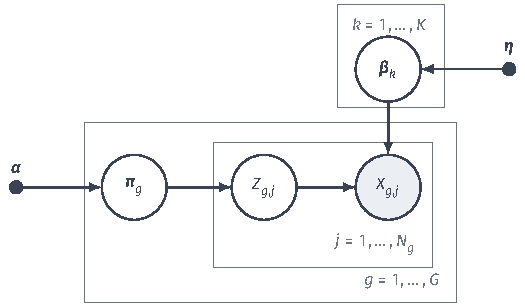
\includegraphics[width=88.935mm]{figures/06-probabilistic-graphical-models/04-models/tikz/pgm-static-directed-plates/figure.pdf}
  \caption{带全局主题先验的LDA重复结构。空心圆表示随机潜在量，填色圆表示观测词，实点表示给定超参数。文档板内每篇有一个$\bm\pi_g$，词板内每词有一组主题分配和观测；$K$个$\bm\beta_k$跨全部文档共享，词节点根据$Z_{g,j}$读取其中一个主题分布。}
  \label{fig:pgm-static-directed-plates}
\end{figure}

若按图~\ref{fig:pgm-static-directed-plates}为主题本身也设置先验，学习对象就改为
\[
 p(\bm\beta_{1:K},\bm\pi_{1:G},\bm z\mid\mathcal D,\bm\alpha,\bm\eta)
 \propto\prod_kp(\bm\beta_k\mid\bm\eta)
      \prod_g p(\bm\pi_g\mid\bm\alpha)
      \prod_{g,j}\pi_{g,z_{g,j}}\beta_{z_{g,j},x_{g,j}}.
\]
这个联合后验保留全局主题的不确定性，不能继续把$\bm\beta$的点参数更新当作同一推断目标。以下用折叠采样直接处理其主题分配。

在主题词分布也有Dirichlet先验的设定下，先积分掉$\bm\pi_g$和$\bm\beta_k$，再使用第~\ref{chap:pgm-sampling}章的Gibbs方法更新一个词的主题。排除当前位置后，文档主题计数记为$n_{g,k}^{-}$，全语料主题词计数为$c_{k,a}^{-}$，并记$c_{k,\cdot}^{-}=\sum_a c_{k,a}^{-}$、$\eta_0=\sum_a\eta_a$，单点条件为
\begin{equation}
  \label{eq:pgm-static-directed-lda-gibbs}
  p(Z_{g,j}=k\mid\text{其余分配},\mathcal{D})
     \propto (n_{g,k}^{-}+\alpha_k)
        \frac{c_{k,x_{g,j}}^{-}+\eta_{x_{g,j}}}
             {c_{k,\cdot}^{-}+\eta_0}.
\end{equation}
文档主题计数给出第一项，主题词计数给出第二项，二者是相应共轭后验的预测权重；文档分母与$k$无关，已经抵消。相乘并归一化，得到精确的单点条件分布。有限轮Gibbs样本构成的整体后验估计仍需考虑抽样误差和混合速度。

实际的一次扫描先从计数表移除当前位置原来的主题贡献，计算式~\eqref{eq:pgm-static-directed-lda-gibbs}的$K$个非负权重，再归一化抽取新主题，并把对应的文档主题计数和主题词计数加回。逐词重复扫描，丢弃初始过渡阶段并检查链的混合后，用保留状态作后验平均。对每个保留分配，可用$\bm\alpha+\bm n_g$与$\bm\eta+\bm c_k$恢复比例和主题的条件Dirichlet后验，再平均所需预测；不能把一个最终分配当成整个后验。

在对称主题先验下，同时置换主题编号和比例坐标，观测分布保持不变。非对称先验可约束部分编号，有限语料中的主题词分布仍可能有其他歧义；相近主题、短文档或过大的主题数会加剧不稳定性。词袋和比例先验各自限制了词序及组间变化，解释主题含义时，需要同时评价这些假设和分解的稳定性。

\subsection{随机成分库及其跨组共享}
\label{sec:pgm-static-directed-random-library}

前面的有限模型先固定可用成分数。现在把总体的成分库也看成未知量：先为一个总体建立随机混合测度，再让多个组共享它提供的原子、拥有不同使用比例。前一个问题由DPM处理，后一个问题再由HDP增加组层；DPM本身仍是单一总体模型。

\subsubsection{DPM：让数据中的占用成分参与推断}
\label{sec:pgm-static-directed-dpm-model}

前面的混合和主题模型都要求事先指定成分（主题）数$K$；$K$过小会欠拟合，过大则浪费容量并增加不稳定性。非参数贝叶斯方法不给成分库设固定上限，而在所有可能成分构成的空间上放置随机概率测度作为先验，使数据实际占用的成分数成为后验推断的一部分。有限混合和主题模型先给定候选成分数$K$。
\term{狄利克雷过程混合}（Dirichlet process mixture, DPM）为混合测度设置随机先验，让有限数据中的占用成分数参与推断。
在标准Borel成分参数空间上，记这个随机概率测度为$G\sim\operatorname{DP}(c,H)$。
其中$c>0$为浓度参数，基测度$cH$的总质量为$c$，$H$是基概率测度。若写作$\operatorname{DP}(\alpha,G_0)$，这里的参数对应为$\alpha=c$、$G_0=H$。
本节采用$c,H$，以区分主题比例先验的参数。
这里需要复用的有限分割规律是：对参数空间的任意有限可测分割$A_1,\ldots,A_m$，随机质量$(G(A_1),\ldots,G(A_m))$服从参数为$(cH(A_1),\ldots,cH(A_m))$的Dirichlet分布；零基质量的单元恒取零。这个规律使计数更新能够同时约束不同分辨率下的成分质量。


无穷多成分、权重总和为1的随机分布不便直接表示，折棒构造（stick-breaking construction）给出一种可数构造：取一根长度为1的棍，第$k$步按一个Beta随机比例从当前剩余棍段上截下一段作为成分$k$的权重，余下部分留给后续成分；反复截取而得的各段长度之和恰为1，由此得到混合建模可用的可数权重序列。
独立抽取$v_k\sim\operatorname{Beta}(1,c)$与$\bm\xi_k\sim H$，依次给剩余质量分配比例$v_k$，令
\[
  w_k=v_k\prod_{\ell<k}(1-v_\ell),\qquad
  G=\sum_{k=1}^{\infty}w_k\delta_{\bm{\xi}_k}.
\]
其中$\delta_{\bm\xi_k}$是原子处的点质量；折棒构造定理保证这个$G$具有上述有限分割规律。
权重和为$1$给出概率测度的归一化，Dirichlet过程分布还依赖这些分割规律。
Teh等的论述介绍了相应构造及其用于层次共享的方式\scite{pgm-static-directed-teh2006}
给定$G$，各记录独立抽取$\bm\zeta_j\mid G\sim G$，再按$\bm X_j\mid\bm\zeta_j\sim p(\cdot\mid\bm\zeta_j)$生成读数。
记录重复抽到一个原子，就使用同一成分参数；成分分布仍可连续。

DPM的学习目标是观测数据下的随机测度和记录分配后验，而非把候选数改大的固定维度最大似然。用$\Pi_{c,H}$表示DP先验律，其目标可写为
\begin{equation}
 p(dG,d\bm\zeta_{1:n}\mid\mathcal D)
 \propto \Pi_{c,H}(dG)\prod_{j=1}^n
       G(d\bm\zeta_j)\,p(\bm x_j\mid\bm\zeta_j).
 \label{eq:pgm-static-directed-dpm-posterior}
\end{equation}
给定读数时，占用成分的证据同时来自已有计数与该成分能否解释当前读数。下面先在成分参数已知的条件下计算DP更新，再把这个结果用于数据条件下的分配。

给定$n$个潜在成分参数，在任意有限分割上，用各单元的计数更新Dirichlet先验。
把这些相容的分割更新合在一起，得到随机测度的后验
\[
  G\mid\bm\zeta_{1:n}\sim\operatorname{DP}
    \left(c+n,\frac{cH+\sum_{j=1}^n\delta_{\bm\zeta_j}}{c+n}\right).
\]
下一条记录的成分参数预测分布由这个后验的均值给出。

取无原子的$H$并积分掉$G$，前$n$个潜在参数中占用成分$k$的计数为$n_k$，下一条复用它的概率为$n_k/(n+c)$，新抽成分的总概率为$c/(n+c)$。已有计数$(3,1)$、$c=1$时，三个选择分别为$0.6,0.2,0.2$。若该条读数也已给定，还需乘各已有成分和基准测度下的预测密度，再归一化。有限$n$至多占用$n$个成分，第$j$次增加成分的先验概率为$c/(c+j-1)$，所以占用数的先验期望是这些概率之和$\sum_{j=1}^n c/(c+j-1)$。可数先验放宽候选容量，实际推断处理当前占用或截断的候选成分，恢复真实有限类别数还需要其他条件。

在$H$与成分似然共轭的情形，可以积分掉$G$及各成分参数，直接更新记录的成分编号。把第$j$条记录移出后，令$n_k^{-j}$为剩余第$k$组的记录数，$\mathcal D_k^{-j}$为其数据。已有成分与新成分的未归一化权重分别是
\begin{equation}
 \begin{aligned}
 a_k&=n_k^{-j}\int p(\bm x_j\mid\bm\xi)
                              p(d\bm\xi\mid\mathcal D_k^{-j}),\\
 a_{\mathrm{new}}&=c\int p(\bm x_j\mid\bm\xi)H(d\bm\xi).
 \end{aligned}
 \label{eq:pgm-static-directed-dpm-allocation}
\end{equation}
先删除移出后变空的成分，再计算各预测密度、归一化这些权重并抽取新编号，最后写回计数与充分统计量；若选中新成分，则创建相应统计量。反复扫描得到占用数和预测分布的后验近似，成分参数需要时再从对应条件后验抽取。这说明$c/(n+c)$只是尚未读取新观测时的新建概率，不能直接用作给定读数后的分配概率。非共轭成分的预测积分可能不能解析完成，须再用数值积分、辅助变量或其他近似，并检查相应采样方法的有效性。

\subsubsection{HDP：使多个组共享同一套可数成分}
\label{sec:pgm-static-directed-hdp-model}

DPM解决了单组数据下成分数不定的问题，但在多组（多篇文档、多个工厂）场景下还有新问题：我们希望各组\emph{共享同一套}主题或成分，只是使用比例不同——不同文档讨论的应是同一批主题，而不是每篇文档各发明一套。若给每组单独抽一个Dirichlet过程，由于基测度连续，各组抽到的成分几乎必然互不相同，无法共享。解决办法是在组之上再加一层：先抽一个全局的随机成分库，再让每组的随机测度围绕这个全局库生成。多个组需要共享成分时，还要让它们使用相同原子。从同一个无原子$H$分别抽取独立Dirichlet过程，各组的原子几乎必然不同。\term{层次狄利克雷过程}（hierarchical Dirichlet process, HDP）取全局浓度参数$\gamma>0$，先抽离散的随机基准，再由它生成组测度：
\begin{equation}
  \label{eq:pgm-static-directed-hdp}
  G_0\sim\operatorname{DP}(\gamma,H),\qquad
  G_g\mid G_0\sim\operatorname{DP}(c,G_0).
\end{equation}
$G_0$几乎必然离散，所以各$G_g$共用同一可数原子集合，同时分别具有组级权重。在主题模型中，这些原子是词分布，每篇文档按自己的权重逐词选择共享主题。一个模型因此同时具有层次共享、混合成员及非固定成分数；这些属性描述不同的组织方式。Teh等进一步说明DP构造和HDP共享原子的机制\scite{pgm-static-directed-teh2006}

HDP的完整生成结构还包括$\bm\zeta_{g,j}\mid G_g\sim G_g$和$X_{g,j}\mid\bm\zeta_{g,j}\sim p(\cdot\mid\bm\zeta_{g,j})$。固定$c,\gamma,H$时，学习目标是全局测度、组测度及各项成分参数的联合后验：
\begin{equation}
 \begin{aligned}
 &p(dG_0,dG_{1:G},d\bm\zeta\mid\mathcal D)\\
 &\quad\propto\Pi_{\gamma,H}(dG_0)
     \prod_g\Pi_{c,G_0}(dG_g)
     \prod_{g,j}G_g(d\bm\zeta_{g,j})p(x_{g,j}\mid\bm\zeta_{g,j}).
 \end{aligned}
 \label{eq:pgm-static-directed-hdp-posterior}
\end{equation}
这里$G$在下标范围$1{:}G$中表示组数，$G_g$表示第$g$组的随机测度。条件于全局库，各组独立抽取权重；观测却会通过未知的全局库联系各组后验。与LDA相比，HDP既推断哪些主题被占用，也推断全局使用倾向怎样约束各文档比例，不能只把它理解为给固定主题数的LDA多加一个普通先验。

为把这个目标变成有限计算，下面在主题词模型中构造一个明确的截断近似。固定截断数$K$，取$v_k\sim\operatorname{Beta}(1,\gamma)$（$k<K$）并令$v_K=1$，把剩余折棒质量合并到最后一项，定义$w_k=v_k\prod_{\ell<k}(1-v_\ell)$。共享原子$\bm\xi_k$在这里是词概率向量，取$H=\operatorname{Dirichlet}(\bm\eta)$。每篇文档的组权重为$\bm\pi_g\mid\bm w\sim\operatorname{Dirichlet}(c\bm w)$，再按$Z_{g,j}\sim\operatorname{Categorical}(\bm\pi_g)$、$X_{g,j}\sim\operatorname{Categorical}(\bm\xi_{Z_{g,j}})$生成词。这个有限模型基于共享原子表示，但$K$有限时不同于原来的可数HDP，必须保留截断敏感性检查。

记全部未知量为$\Omega=(\bm v,\bm\xi,\bm\pi,\bm z)$，上述步骤对应明确的联合密度
\begin{equation}
 \begin{aligned}
 p_K(\mathcal D,\Omega)
 ={}&\prod_{k<K}\operatorname{Beta}(v_k;1,\gamma)
       \prod_{k=1}^K\operatorname{Dirichlet}(\bm\xi_k;\bm\eta)\\
 &\cdot\prod_g\operatorname{Dirichlet}(\bm\pi_g;c\bm w)
       \prod_{g,j}\pi_{g,z_{g,j}}\xi_{z_{g,j},x_{g,j}}.
 \end{aligned}
 \label{eq:pgm-static-directed-hdp-truncated-joint}
\end{equation}
采用平均场$q(\Omega)=\prod_{k<K}q(v_k)\prod_kq(\bm\xi_k)\prod_gq(\bm\pi_g)\prod_{g,j}q(Z_{g,j})$，其中折棒因子为Beta，词分布与组权重因子为Dirichlet，分配因子为类别分布。所有形状参数保持正值。具体的优化目标是
\begin{equation}
 \max_q\;\mathcal L_K(q)
   =\mathbb E_q[\log p_K(\mathcal D,\Omega)-\log q(\Omega)].
 \label{eq:pgm-static-directed-hdp-elbo}
\end{equation}
它下界化的是有限模型的$\log p_K(\mathcal D)$；提高该下界不能直接证明原可数模型的证据提高。这里把第~\ref{chap:pgm-variational}章的变分原理用于刚才写出的有限联合模型，不把以下计算称为原HDP的解析后验。

令$q(\bm\pi_g)=\operatorname{Dirichlet}(\bm a_g)$、$q(\bm\xi_k)=\operatorname{Dirichlet}(\bm\lambda_k)$、$q(Z_{g,j}=k)=r_{g,j,k}$。固定其余因子时，分别收集联合对数密度中含当前变量的项，可得
\begin{equation}
 \begin{aligned}
 r_{g,j,k}&\propto\exp\{\mathbb E_q\log\pi_{g,k}
                          +\mathbb E_q\log\xi_{k,x_{g,j}}\},\\
 a_{g,k}&=c\mathbb E_q[w_k]+\sum_jr_{g,j,k},\\
 \lambda_{k,a}&=\eta_a+\sum_{g,j}r_{g,j,k}\mathbb I\{x_{g,j}=a\}.
 \end{aligned}
 \label{eq:pgm-static-directed-hdp-local-vi}
\end{equation}
第一行对$k$归一化；两类对数期望与LDA一样由digamma差计算。组权重更新的先验伪计数是$c\mathbb E_q[w_k]$，而不是每组各自固定的一组$\alpha_k$；共享主题更新则汇集所有文档的词频。若$q(v_k)=\operatorname{Beta}(u_k,b_k)$，独立性给出$\mathbb E_q[w_k]=\mathbb E_q[v_k]\prod_{\ell<k}\mathbb E_q[1-v_\ell]$，其中$\mathbb E_q[v_k]=u_k/(u_k+b_k)$、$v_K=1$。

全局折棒的更新不能直接套用LDA计数公式。组先验的对数密度中包含以下依赖全局权重的项：
\[
 -\sum_k\log\Gamma(cw_k).
\]
它使全局权重与组权重之间不再共轭。固定其他变分因子后，可对Beta形状参数的对数$\bm\omega=(\log u_k,\log b_k)_{k<K}$数值优化$\mathcal L_K$。例如把其他因子的期望先汇总，记$A(\bm v)=\mathbb E_{q(\Omega\setminus\bm v)}\log p_K(\mathcal D,\Omega)$，在微分与积分可交换、梯度估计方差有限时，有
\[
 \nabla_{\bm\omega}\mathcal L_K
 =\mathbb E_{q_{\bm\omega}(\bm v)}
 [(A(\bm v)-\log q_{\bm\omega}(\bm v))
                     \nabla_{\bm\omega}\log q_{\bm\omega}(\bm v)].
\]
抽取折棒样本、计算括号内的全局与组先验项，再平均梯度并更新$\bm\omega$，就是前文评分函数估计在这个模型中的一项实现。概率接近边界时要检查数值精度和梯度方差；有限样本梯度更新不保证每一步ELBO上升。

完整训练循环因而包含：更新各词分配，汇总组权重与共享主题的参数，再优化全局折棒因子；随后回到各文档重算分配。初始化时使用正的形状参数，局部更新可多次迭代；停止时同时检查ELBO估计的变化及其蒙特卡洛波动，而不是仅比较相邻两次带噪数值。增大$K$后重新检查预测和尾部质量敏感性，分别报告截断近似、平均场近似与数值优化的限制。给已有文档预测新词，可用$\sum_k\mathbb E_q[\pi_{g,k}]\mathbb E_q[\xi_{k,a}]$；新文档则先从学得的全局权重及共享主题构造组先验，再结合其已观测词做局部推断。

DPM和HDP把有限数据占用的成分数、分配与随机权重纳入后验推断。以上演示固定浓度等超参数；若还要估计这些量，需要另加经验贝叶斯目标，或为它们设先验后扩大联合后验。截断变分用有限候选近似可数模型，需要检查截断误差；采样调整占用成分，需要检查链的混合。HDP还要共同处理组级成分和全局原子的关系，独立拟合各组有限混合无法完成这项共享推断。浓度参数影响分组倾向，需结合超参数估计和预测检验使用。输出时可报告预测、占用数及组间共享的不确定性，原子编号本身仍只承担命名。

\section{结构组合与查询选择}
\label{sec:pgm-static-directed-comparison}

本章模型沿两个维度变化：潜变量取值离散或连续，共享发生在记录内或跨组。比较时固定三条线索：面对一个查询，模型要对哪些随机量求和或积分、这些量在什么范围内共享、哪些非唯一性会限制对结果的解释；先固定查询与被积分的随机量，才能在同一口径下比较计算代价和适用场景。在表~\ref{tab:pgm-static-directed-comparison}中，给定所选全局参数或超参数，按各模型的设定汇总随机潜在量，得到观测似然$p(\bm x)$；用点估计固定的参数不再积分。NB和TAN的完整训练记录为$(y,\bm x)$，类别预测时则对$Y$归一化。独立性、共享和非唯一性另列，便于分析同一种查询在不同结构中需要完成哪些工作。

\begin{table*}[htbp]
  \centering
  \small
  \begin{tabularx}{\linewidth}{@{}
    >{\raggedright\arraybackslash}p{28mm}
    >{\raggedright\arraybackslash}p{30mm}
    >{\raggedright\arraybackslash}p{27mm}
    >{\raggedright\arraybackslash}p{30mm}
    >{\raggedright\arraybackslash}X@{}}
    \toprule
    模型与潜在量 & 独立性与共享 & 观测似然 & 局部后验 & 非唯一性与主要代价\\
    \midrule
    NB／TAN：训练时无潜变量 &
    类内独立／类内树；参数跨样本共享 &
    完整记录直接乘积 &
    类别后验枚举$K$项 &
    支持不足的条件表不确定；TAN还需选择树\\
    自回归：无随机潜变量 &
    顺序父集；条件网络可共享参数 &
    条件密度直接乘积 &
    前缀续写直接；任意补全未必易算 &
    网络参数可不唯一；优化、顺序选择与串行生成\\
    有限混合：离散分配 &
    样本在固定参数下独立；类内结构由成分决定 &
    $K$项有限和 &
    成分责任度精确 &
    标签交换、冗余成分；局部极值与退化\\
    FA／PPCA：连续因子 &
    给定因子后观测独立；共享载荷 &
    解析高斯密度 &
    解析高斯后验与缺失预测 &
    旋转及可能的额外分解歧义；维数与噪声假设\\
    LDA：连续比例与离散主题 &
    组级比例、全局主题；组内条件独立 &
    需积分比例，通常近似 &
    联合后验通常近似，局部条件可解析 &
    主题置换与重叠；局部推断和全局学习交替\\
    DPM／HDP：分配与随机测度 &
    可数候选成分；HDP跨组共享原子 &
    对未知随机量积分通常需近似 &
    采样或截断变分 &
    成分编号不唯一；占用数、超参数与近似误差\\
    \bottomrule
  \end{tabularx}
  \caption{静态有向模型在给定参数或超参数下的计算。表中的精确结果指相应有限求和、解析积分或局部条件；学习目标、参数不确定性及潜在解释另按各模型分析。}
  \label{tab:pgm-static-directed-comparison}
\end{table*}

直接模型以局部条件拟合观测联合分布。NB用类内独立减少待估参数，TAN增加树边及结构搜索，神经自回归则用非线性条件与参数共享扩大可表达的关系。完整记录可直接计算局部乘积，祖先生成和缺失查询还需按各自依赖进行。潜变量路线也可能保留精确计算：有限混合显式汇总$K$项，线性高斯模型解析积分，同时给出似然和局部后验。

共享随机量会联系不同位置的推断。pLSA固定文档比例时，逐词做有限求和；LDA积分共同的文档比例后，主题分配需要一起解释这些词。全局主题再带先验时，不同文档也相互联系，HDP还需要推断共享的占用成分。这些联系决定了联合后验的规模，除各变量的状态数外，还需考察它们共同读取哪些数据。

模型之间的联系还要落到结构和学习对象的变化上。NB与TAN都保留类别生成属性的结构，TAN只放宽类内父集；把NB的训练类别隐藏，并保留原来的条件乘积，就得到乘积分布的有限混合。这里改变的是类别的观测状态，所以已知计数变成需要E步计算的后验期望计数。FA到PPCA则没有改变观测状态，而是把逐维噪声约束为同一个方差；两者都约束协方差的低秩加噪声分解。下一章的高斯马尔可夫随机场将转而约束精度矩阵的零元素，二者对同一高斯分布族施加不同结构限制。自回归网络的三种实现都保留顺序条件乘积，掩码和卷积改变条件函数的计算及参数共享。

有限混合与混合成员的区别在分配单位：前者一条记录选择一个成分，后者在一组内部逐项选择。pLSA到LDA进一步把文档比例由固定参数变为随机量，因此新文档有了比例先验，也增加了比例积分。DPM对单一总体引入随机成分库；HDP在这个库之上增加组权重，让不同组共享原子而保持不同使用比例。这些变化分别作用于容量、共享和分配单位，不能排成一条每个模型都替代前者的升级链。

表~\ref{tab:pgm-static-directed-learning-map}补充各分支的目标和更新对象，与表~\ref{tab:pgm-static-directed-comparison}的查询成本合读，可以区分“模型怎样表示”“参数怎样学到”和“训练后怎样使用”。
\begin{table*}[htbp]
 \centering\small
 \begin{tabularx}{\linewidth}{@{}p{25mm}XXX@{}}
 \toprule
 模型 & 结构改变与动机 & 学习目标 & 具体更新对象\\
 \midrule
 NB／TAN & 类内独立或属性树减少条件表规模 & 带标签联合似然；TAN另选树 & 类别与父配置计数；条件互信息最大生成树\\
 NADE／MADE／PixelCNN & 前缀复用、掩码与空间共享控制条件函数 & 完整记录自回归负对数似然 & 由各位置梯度共同更新网络权重\\
 有限混合／GMM & 用未知离散成分解释多种模式 & 成分求和后的观测似然 & 责任度、加权均值与协方差交替更新\\
 FA／PPCA & 连续共同强度与独有噪声分解相关 & 低秩加噪声高斯似然 & 后验一、二阶矩，载荷与受约束噪声\\
 层次正态 & 组参数共享总体且保留差异 & 组边缘似然或联合后验 & 组后验矩与超参数；或联合采样、变分\\
 pLSA／LDA & 逐词分配；固定或随机文档比例 & pLSA似然、LDA的ELBO或联合后验 & 文档比例、主题词频；LDA另推断比例或折叠分配\\
 DPM／HDP & 随机成分库；HDP跨组共享原子 & 随机测度联合后验；有限近似的ELBO & 分配、成分、组权重及全局权重\\
 \bottomrule
 \end{tabularx}
 \caption{建模选择与学习计算的对应。表中并列的目标属于不同设定，使用某一模型时须先选定点参数估计或贝叶斯后验目标，再采用相应更新。}
 \label{tab:pgm-static-directed-learning-map}
\end{table*}

也可以组合上述属性。混合因子分析为每个离散成分配置连续因子，成分内积分后仍是低秩加对角协方差的高斯，所以成分责任度和因子后验可解析计算。自回归条件可采用有限混合，组级载荷可设置层次先验。因此离散或连续、线性高斯或非线性、组间共享或独立、逐项生成或联合生成，分别描述模型的一项选择。

观测分布估计准确时，潜在解释仍可能受对称性约束：网络权重可有多种表示，成分可交换编号，因子可旋转方向。选择模型时，可先用留出数据评价预测，再按目的检查所需输出；解释结构需要报告对称性及稳定性，补全任务则需要评价条件预测和误差范围。似然计算、预测表现和潜在语义各有相应的核验对象。

\section{本章小结}
\label{sec:pgm-static-directed-summary}

本章把表示、推断和学习组装到具体的静态有向模型上，并沿三条主线展开：观测之间的直接依赖、记录内部由潜变量给出的共同解释、以及跨记录跨组的共享。静态有向分解把局部条件组合成联合分布。全部变量可观测时直接读取乘积，引入潜在状态后则先汇总它们，得到观测分布。两个传感器的同一联合表可用自回归条件或隐藏类别的混合表示，前者给出读数预测次序，后者加入需要另行验证的工作状态解释。

有限混合用责任度与成分参数交替学习，固定参数的局部后验仍可精确求得。线性高斯积分把观测协方差、降维和缺失预测联系起来；共享随机量与混合成员联系多个记录或组的推断，联合计算可能需要近似。取值类型与共享方式可以组合使用，标签置换、因子旋转和其他分解歧义则限制了潜在坐标的唯一解释。

判断新模型时，可以从联合归一化、查询待消变量、共享范围和估计的边界条件逐项展开。若建模依据首先是变量状态之间的相容性，可以改用局部相容函数与统一归一化，而不必先指定谁生成谁。第~\ref{chap:pgm-energy-models}章据此比较联合归一化与输出条件归一化；这是一种表示选择，不意味着有向分解不能表达对称的观测分布。第~\ref{chap:pgm-generative}章再以自回归和高斯潜变量为参照，讨论神经网络如何参数化更灵活的密度，以及相应概率计算的代价。

\paragraph{扩展阅读}
Bishop的PRML用混合、潜变量及变分学习展开静态模型，Koller与Friedman从局部条件结构讨论共同的推断与学习方法。可沿同一图的作用域比较不同局部分布，检查哪些求和或积分仍有解析形式，哪些学习目标需要近似后验\scite{bishop2006,pgm-koller2009}
